\documentclass[11pt,a4paper]{article}

\usepackage[margin=1in]{geometry}
\usepackage{graphicx}
\usepackage[hidelinks]{hyperref}
\usepackage{parskip} 
\usepackage{titlesec}
\usepackage{mathptmx}
\usepackage{xcolor}
\usepackage{fancyhdr}
\usepackage{enumitem}
\usepackage{caption} 

\titleformat{\section}{\normalfont\Large\bfseries\color{blue}}{\thesection}{1em}{}
\titleformat{\subsection}{\normalfont\large\bfseries\color{blue!80!black}}{\thesubsection}{1em}{}

\pagestyle{fancy}
\fancyhf{}
\fancyhead[L]{Major Assignment - SCL | Maxmudov Kamran}
\fancyhead[R]{\thepage}
\renewcommand{\headrulewidth}{0.4pt}

\let\oldincludegraphics\includegraphics
\renewcommand{\includegraphics}[2][]{%
  \begin{center}
    \oldincludegraphics[#1]{#2}
  \end{center}
}

\begin{document}

\tableofcontents
\newpage

\setcounter{section}{-1}
\section{Introduction}

\subsection{Overview}

In today's digital era, where information is abundant and constantly evolving, it becomes essential to transform theoretical knowledge into practical skills. This report focuses on applying foundational knowledge of \textbf{Computer Networks} through practical simulations. Utilizing Cisco Packet Tracer, I explore virtual network design and configuration. In the final part, I consider a real-world scenario involving a company that requires network planning by a qualified professional.

\subsection{Cisco Packet Tracer}

\textbf{Cisco Packet Tracer} is a powerful network simulation tool developed by Cisco. It enables users—students and professionals alike—to design, configure, and troubleshoot networks without needing physical devices.

\textbf{Key Features:}
\begin{itemize}[leftmargin=1.5em]
    \item \textbf{Network Simulation} – Emulates routers, switches, end devices, and IoT components.
    \item \textbf{Realistic Configuration} – Offers CLI-based setup similar to real Cisco hardware.
    \item \textbf{Packet Analysis} – Allows users to visualize packet flow within a network.
\end{itemize}

\section{Activity 1 – Configuring a Wireless Router}

\subsection{Concept Overview}

A \textbf{wireless router} allows devices to connect to a network without using cables. It functions as both an access point and a gateway to the internet or local resources. In this simulation, I configure a wireless router in Cisco Packet Tracer, set up Wi-Fi with WPA2 security, enable DHCP, and connect a laptop wirelessly to verify network functionality.

\subsection{Simulation Steps}

\begin{enumerate}
\item \textbf{Added Devices:} I placed a wireless router and a laptop in the workspace.

\fbox{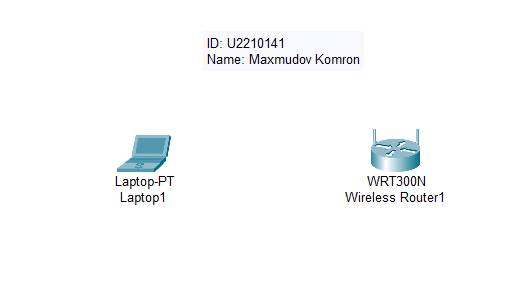
\includegraphics[width=0.8\textwidth]{Images/1.1.png}}

\item \textbf{Configured SSID and Security:} I assigned the SSID “Activity1-WiFi” and set WPA2-PSK with a strong password.

\fbox{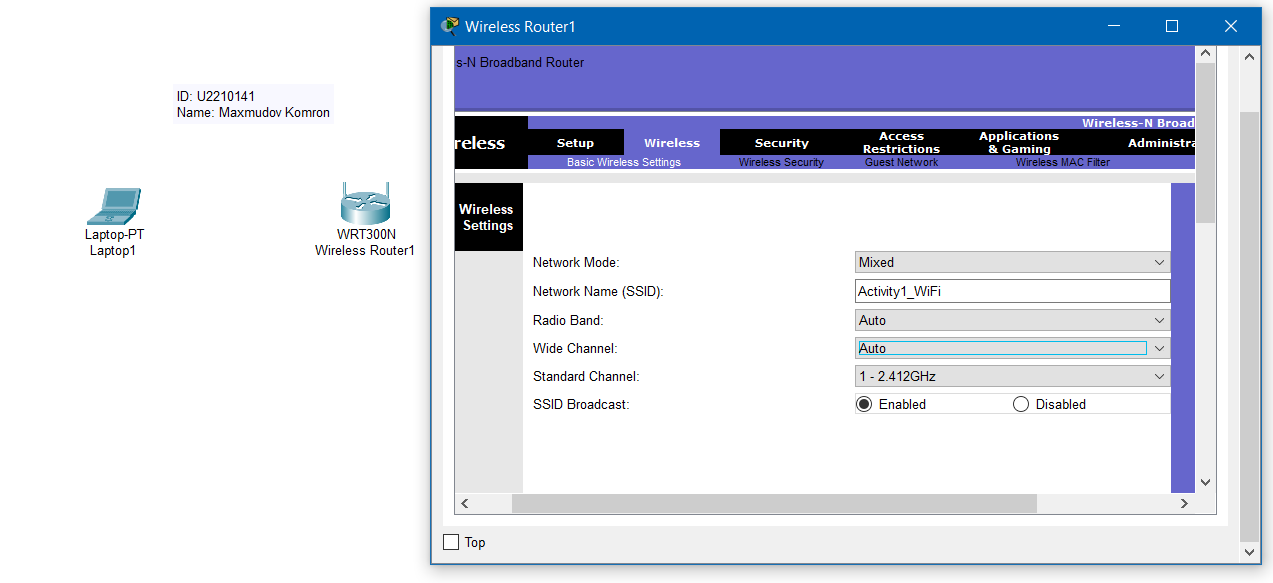
\includegraphics[width=0.8\textwidth]{Images/1.2.1.png}} \\[1em]
\fbox{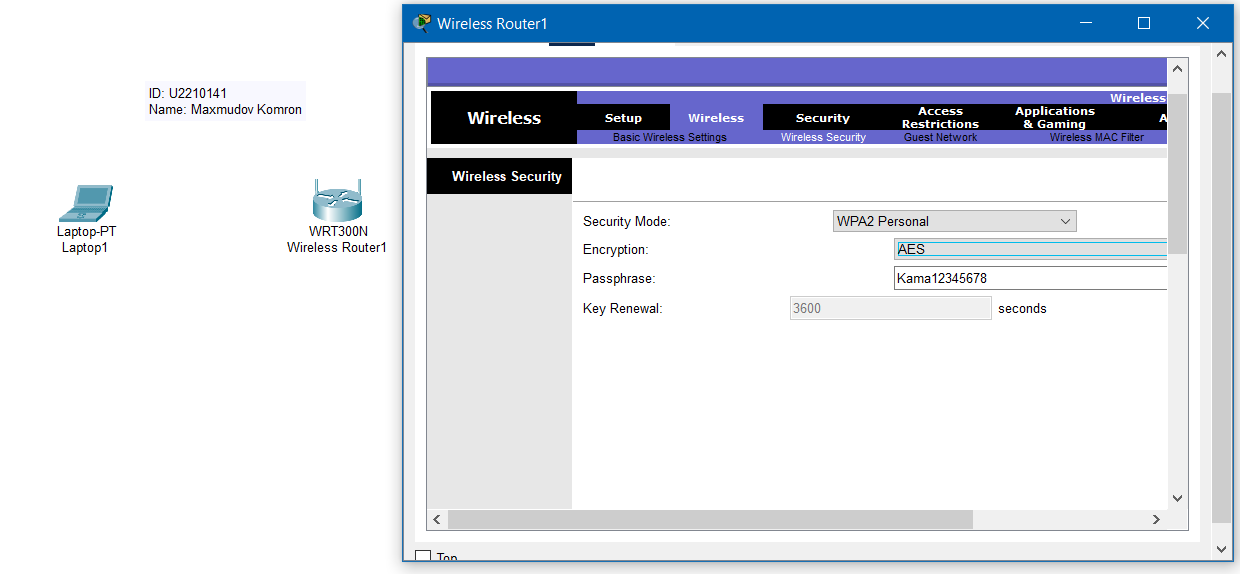
\includegraphics[width=0.8\textwidth]{Images/1.2.2.png}}

\item \textbf{Enabled DHCP:} DHCP was enabled on the router to assign IP addresses dynamically.

\fbox{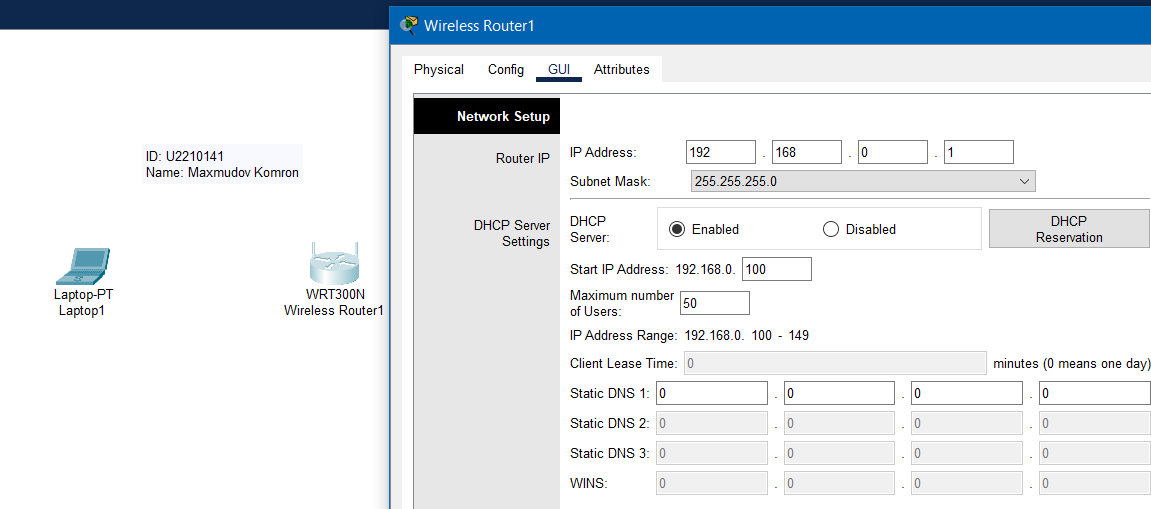
\includegraphics[width=0.8\textwidth]{Images/1.3.png}}

\item \textbf{Connected Laptop to Wi-Fi:} The laptop was connected to the network by selecting the SSID and entering the password.

\fbox{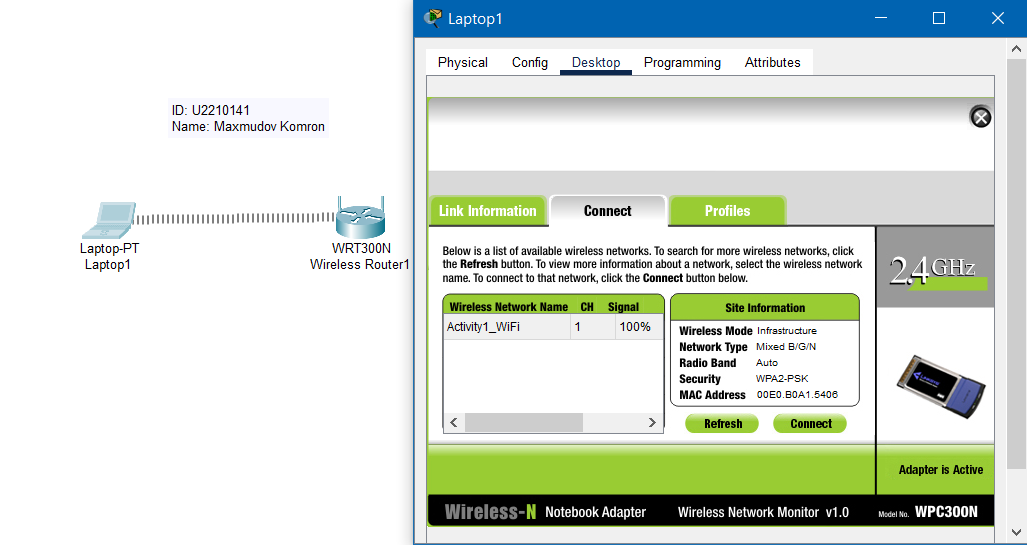
\includegraphics[width=0.8\textwidth]{Images/1.4.png}}

\item \textbf{Verified IP Address:} The laptop received an IP address from the router, confirming a successful connection.

\fbox{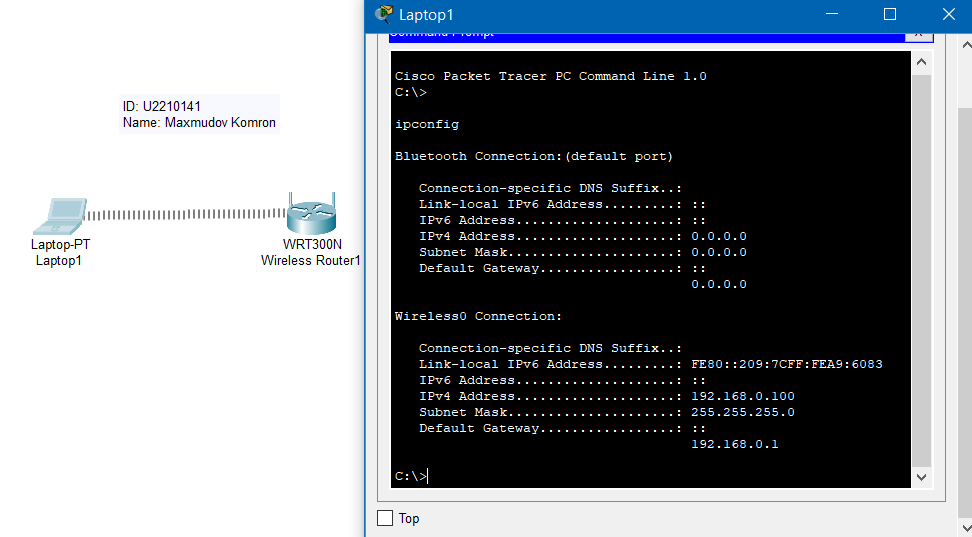
\includegraphics[width=0.8\textwidth]{Images/1.5.png}}

\item \textbf{Tested Connectivity:} I pinged the router from the laptop, and received replies — confirming a working wireless link.

\fbox{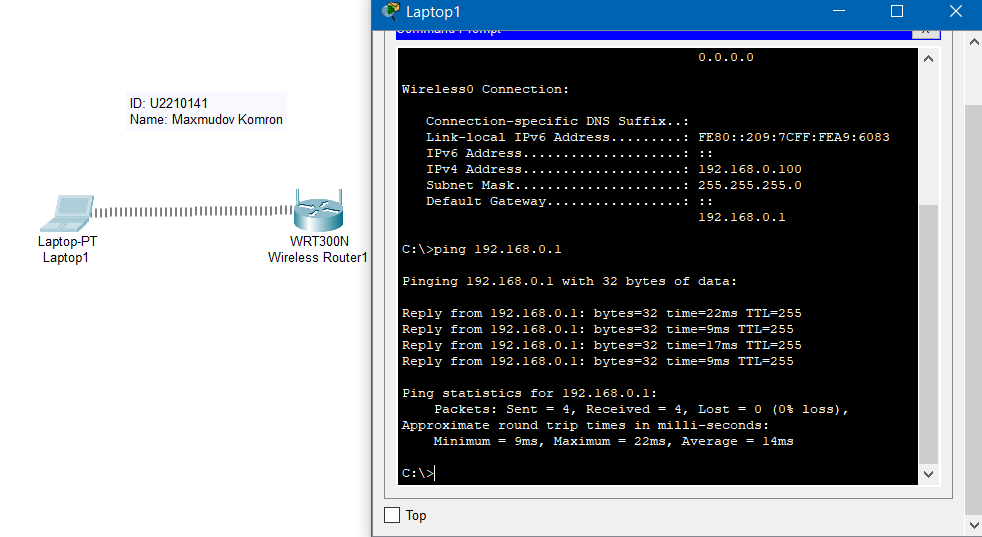
\includegraphics[width=0.8\textwidth]{Images/1.6.png}}
\end{enumerate}

\subsection{Summary}

I successfully configured a wireless router with secure settings and DHCP, connected a laptop via Wi-Fi, and verified both IP allocation and connectivity. This simulation models a standard home or small-office wireless setup.

\section{Activity 2 – Configuring WLAN using Packet Tracer}

\subsection{Concept Overview}

A \textbf{Wireless Local Area Network (WLAN)} allows devices to connect wirelessly within a specific range, using Wi-Fi standards. In this simulation, I will configure a WLAN using Cisco Packet Tracer, set up a wireless router as the access point, define the wireless network (SSID), enable security features, and connect multiple devices to verify network functionality.

\subsection{Simulation Steps}

\begin{enumerate}
\item \textbf{Added Devices:} I placed the wireless router, two laptops, and a desktop in the Packet Tracer workspace.

\fbox{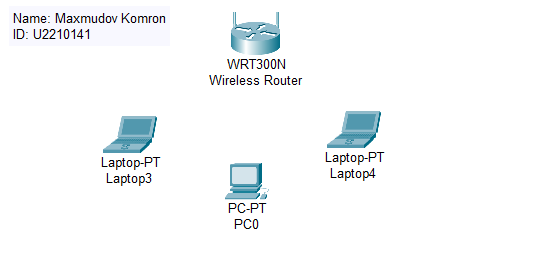
\includegraphics[width=0.8\textwidth]{Images/2.1.png}}

\item \textbf{Set SSID and Wireless Security:} I created the SSID "Activity2-WiFi" and applied WPA2-PSK security with a secure password to prevent unauthorized access.

\fbox{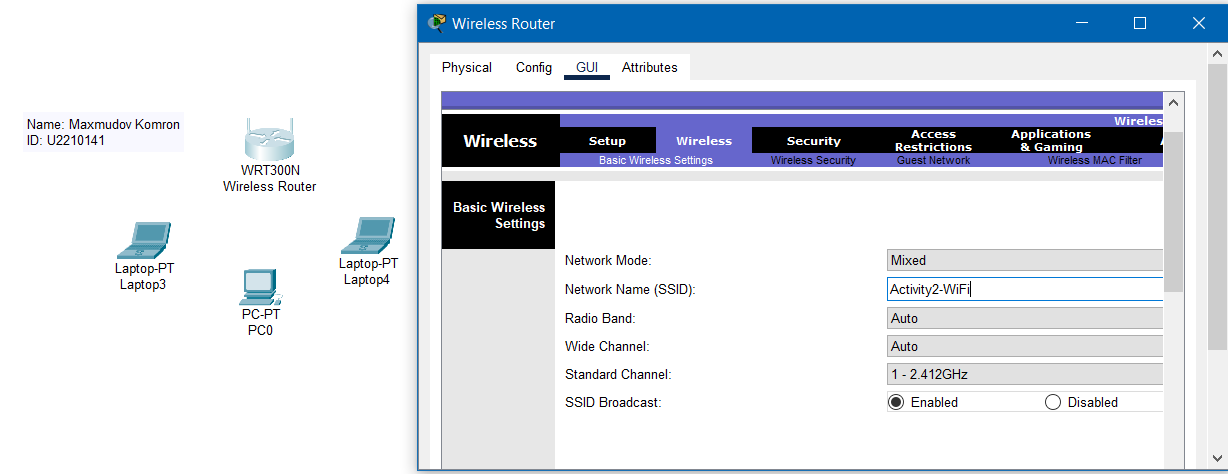
\includegraphics[width=0.8\textwidth]{Images/2.2.png}} \\[1em]
\fbox{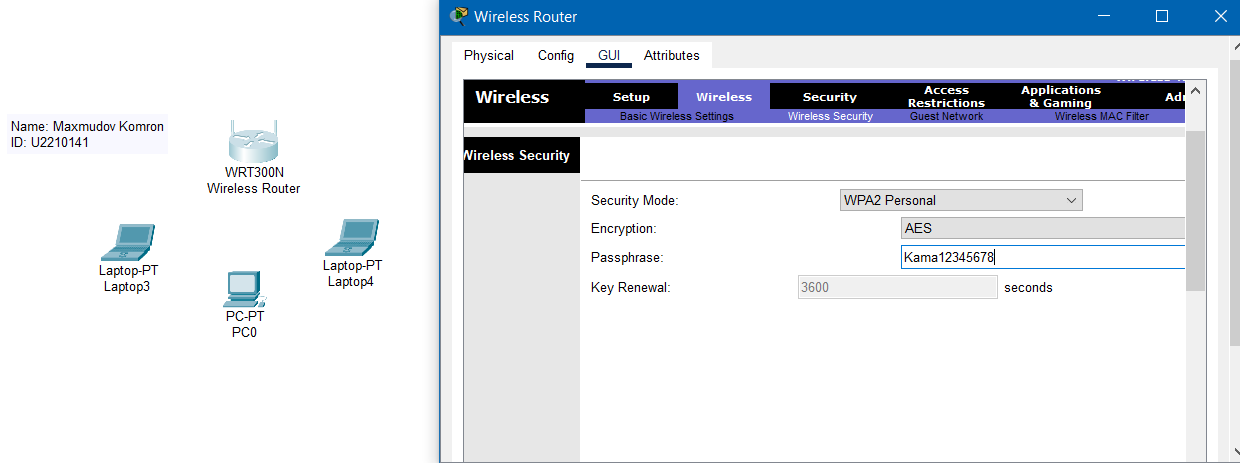
\includegraphics[width=0.8\textwidth]{Images/2.3.png}}

\item \textbf{Enabled DHCP on Router:} I enabled DHCP on the wireless router to automatically assign IP addresses to the connected devices.

\fbox{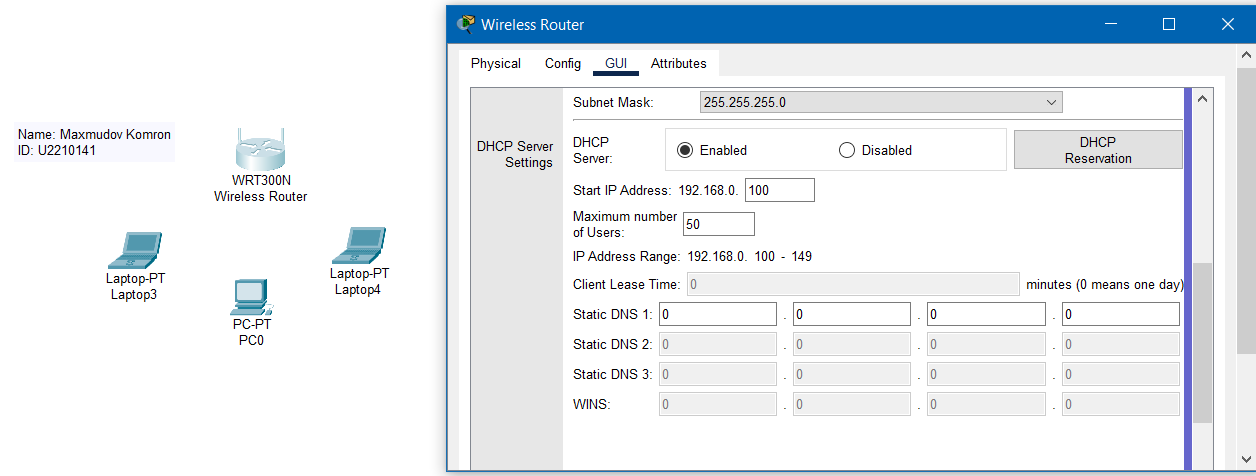
\includegraphics[width=0.8\textwidth]{Images/2.4.png}}

\item \textbf{Connected Devices to WLAN:} I connected the two laptops to the wireless network by selecting the SSID and entering the WPA2 password. The desktop was connected via a wired Ethernet connection because, in Packet Tracer, PCs do not have wireless network adapters, and they can only connect via wired connections.

\fbox{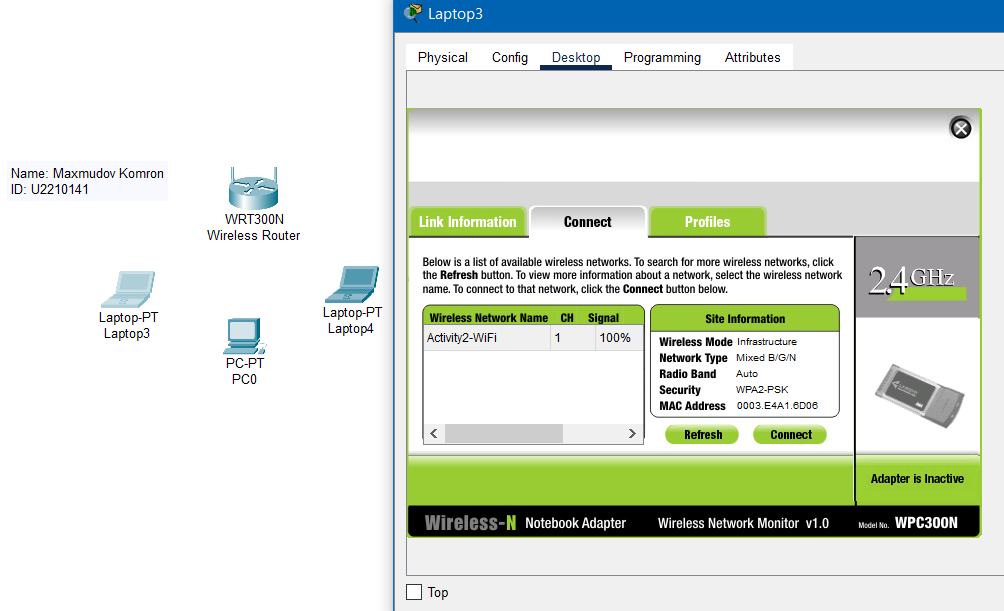
\includegraphics[width=0.8\textwidth]{Images/2.5.1.png}} \\[1em]
\fbox{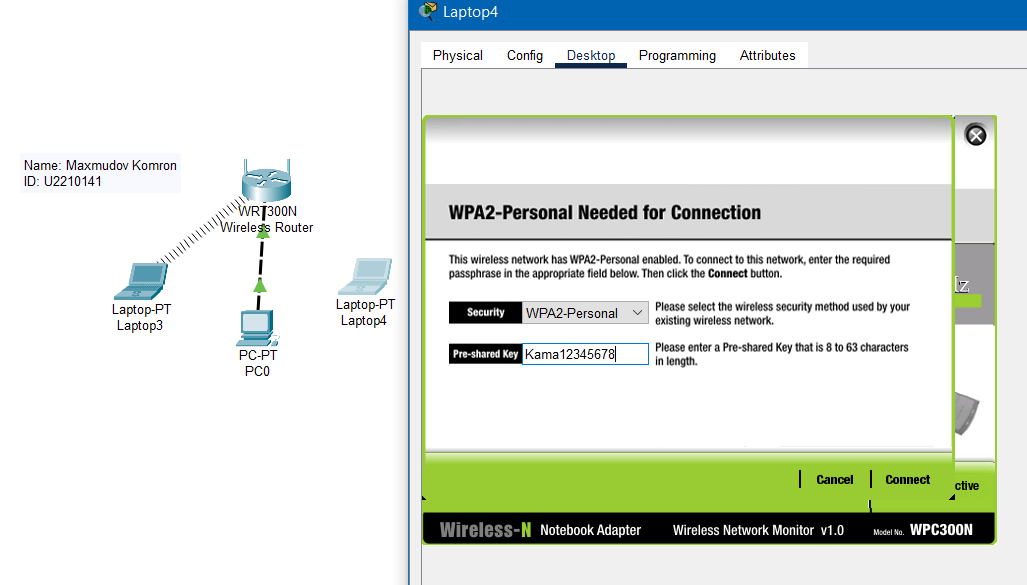
\includegraphics[width=0.8\textwidth]{Images/2.5.2.png}}

\item \textbf{Verified IP Address Assignment:} I checked that all connected devices received an IP address from the router, confirming they were successfully connected to the WLAN (for laptops) and wired network (for the desktop).

\fbox{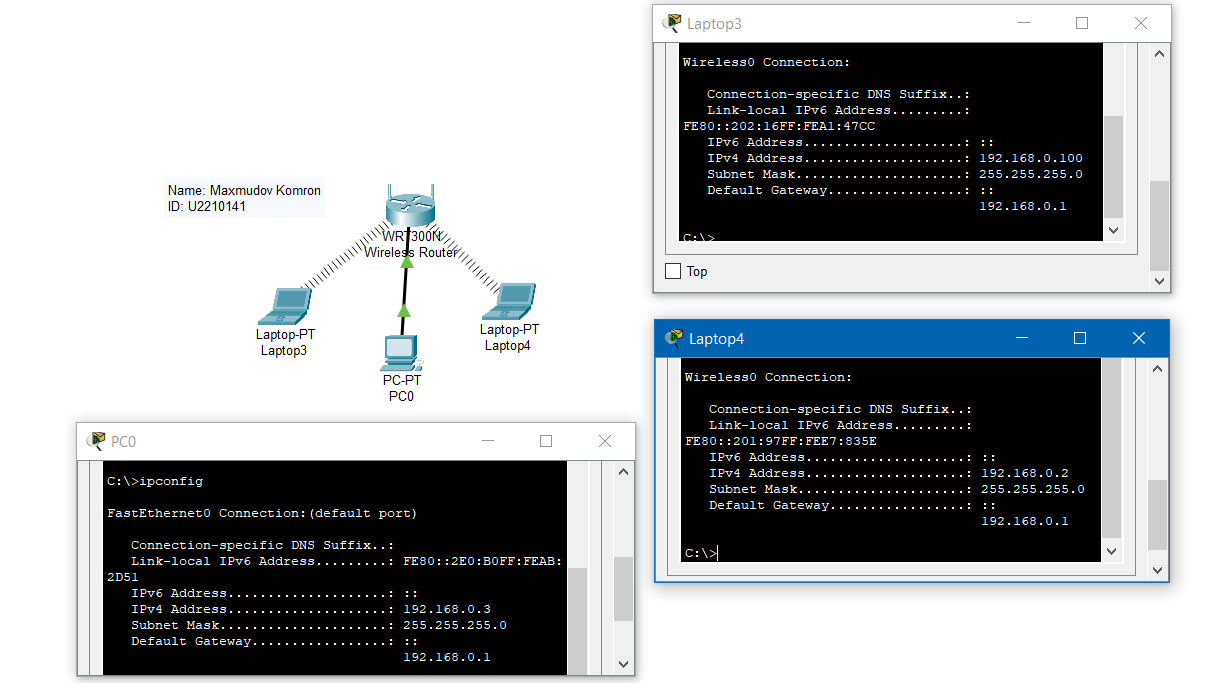
\includegraphics[width=0.8\textwidth]{Images/2.6.png}}
\end{enumerate}

\subsection{Summary}

In this activity, I successfully configured a WLAN by setting up a wireless router as an access point, securing the network with WPA2 encryption, enabling DHCP for automatic IP address assignment, and connecting multiple devices to the network. The laptops were connected via Wi-Fi, while the desktop was connected via a wired Ethernet connection. The desktop was connected through a wire because Packet Tracer does not support wireless network adapters for PCs, so the only option for connecting PCs is through a wired connection.

\section{Activity 3 – Configuring DHCP on Router using Cisco Packet Tracer}

\subsection{Concept Overview}

A \textbf{Dynamic Host Configuration Protocol (DHCP)} server allows devices on a network to automatically obtain IP addresses and other network configuration settings. In this activity, I will configure a router to function as a DHCP server in Cisco Packet Tracer. The router will dynamically assign IP addresses to devices on the network, eliminating the need for manual IP address configuration.

\subsection{Simulation Steps}

\begin{enumerate}
\item \textbf{Added Devices and Configured Router:} I placed a router, a switch, and several end devices in the Packet Tracer workspace.

\fbox{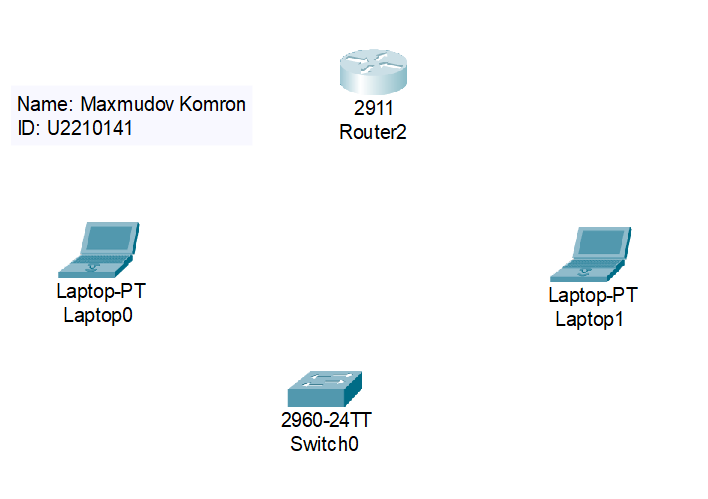
\includegraphics[width=0.8\textwidth]{Images/3.1.png}}

\item \textbf{Configured DHCP Pool and Enabled DHCP on Interface:} I defined the DHCP pool with a network range (e.g., \texttt{192.168.1.0} to \texttt{192.168.1.255}), set the router’s IP address (\texttt{192.168.1.1}) as the default gateway, and configured DHCP to assign IP addresses within this range. DHCP was enabled on the router's \texttt{GigabitEthernet 0/0} interface to allow devices to automatically receive their IP addresses and network settings.

\fbox{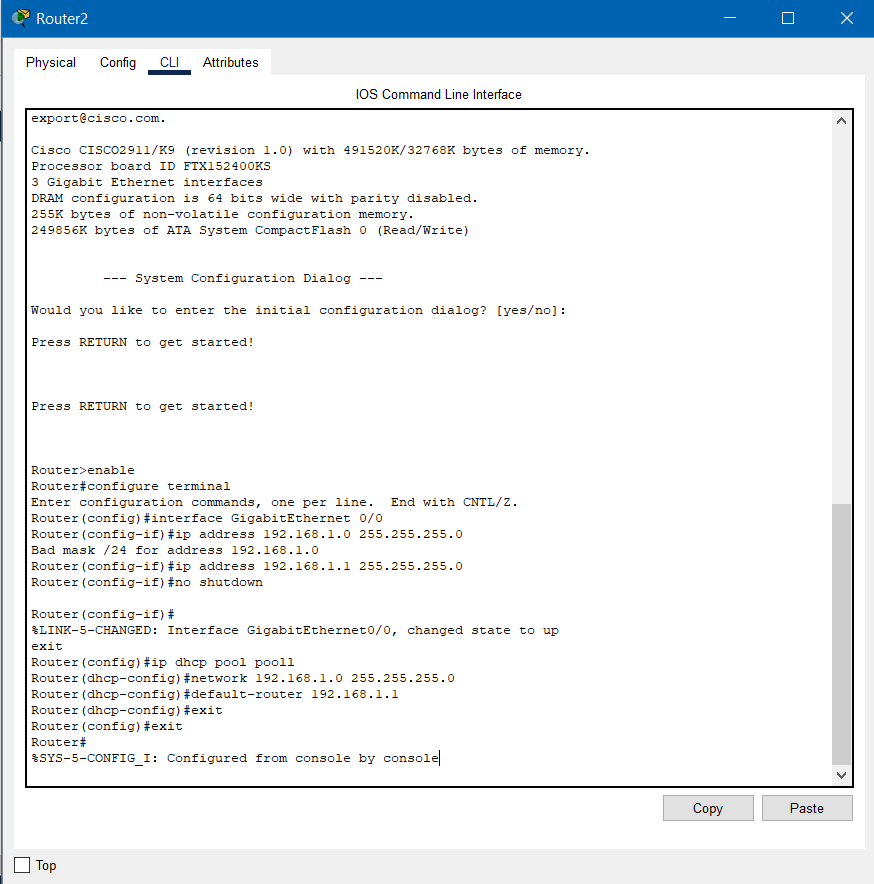
\includegraphics[width=0.8\textwidth]{Images/3.2.png}}

\item \textbf{Connected Devices to the Network:} I connected the devices to the switch, ensuring they were in the same network as the router. The devices were set to receive their IP addresses automatically from the router.

\fbox{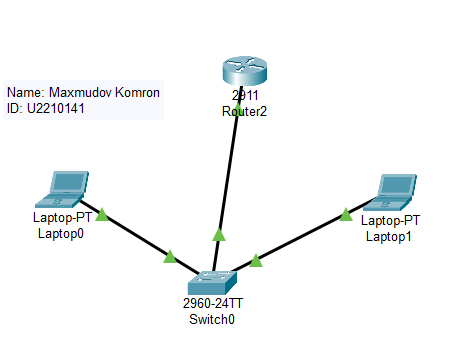
\includegraphics[width=0.8\textwidth]{Images/3.3.png}}

\item \textbf{Verified IP Address Assignment:} I opened the IP configuration settings on each device and set them to obtain an IP address automatically via DHCP. This allowed the devices to request IP addresses from the router’s DHCP server.

\fbox{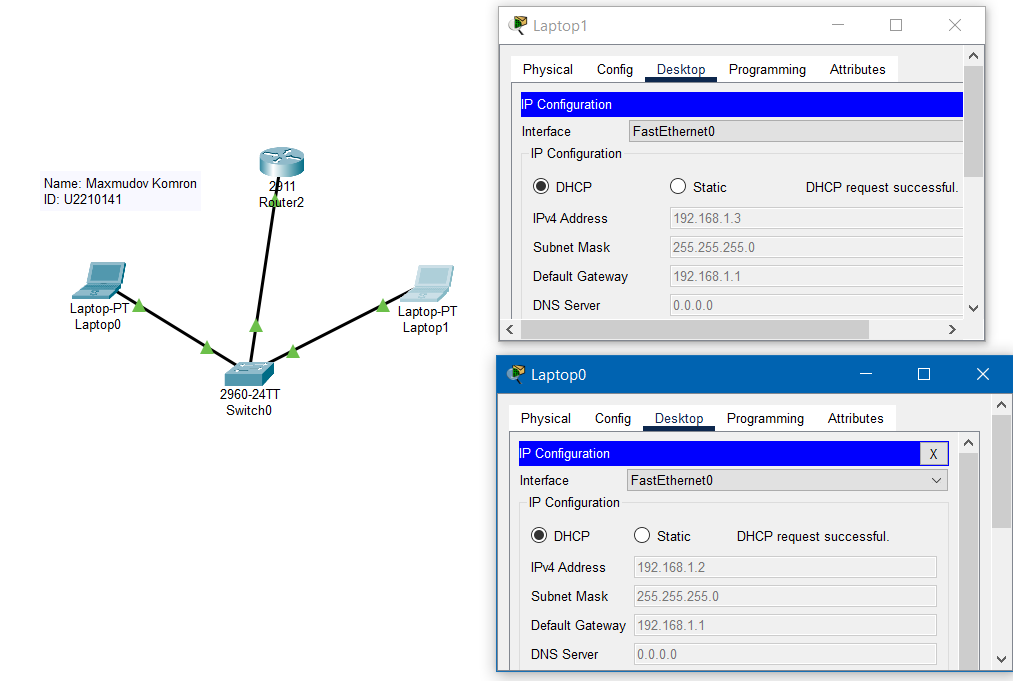
\includegraphics[width=0.8\textwidth]{Images/3.4.png}}

\item \textbf{Tested Connectivity:} I performed a ping test between devices to verify that all devices were successfully connected to the network and were receiving proper IP addresses.

\fbox{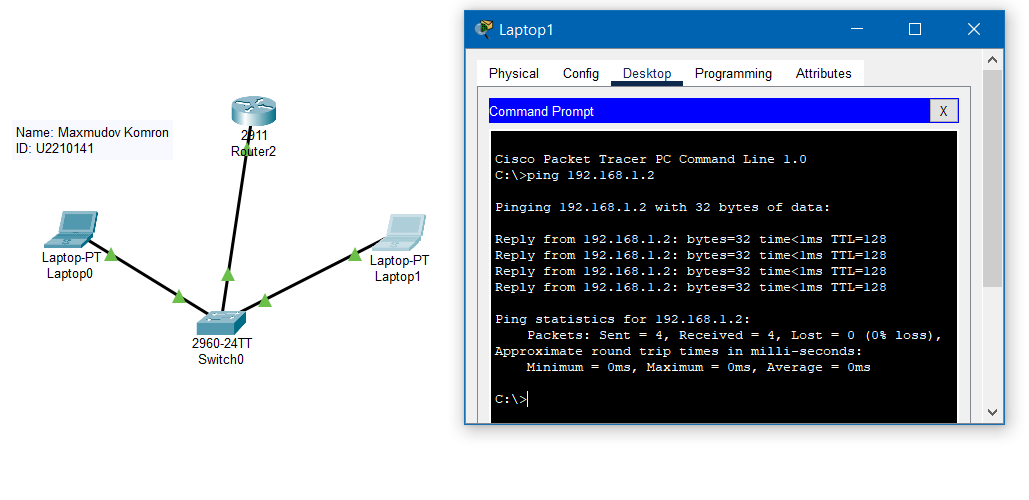
\includegraphics[width=0.8\textwidth]{Images/3.5.png}}
\end{enumerate}

\subsection{Summary}

In this activity, I successfully configured a router as a DHCP server, which dynamically assigned IP addresses to devices on the network. Devices were connected to the network and received IP addresses via DHCP. Connectivity was verified using ping tests between devices.

\section{Activity 4 – Configuring a Dedicated DHCP Server using Cisco Packet Tracer}

\subsection{Concept Overview}

A \textbf{Dedicated DHCP (Dynamic Host Configuration Protocol) Server} is a standalone device or service responsible for automatically assigning IP addresses and other network settings to client devices. Unlike a router-based DHCP configuration, using a dedicated DHCP server allows for more centralized management and scalability. In this activity, I configured a DHCP server device in Cisco Packet Tracer to handle IP address distribution for devices connected to a network.

\subsection{Simulation Steps}

\begin{enumerate}
\item \textbf{Added Devices and Network Topology:} I placed a DHCP server, a router, a switch, and several end devices (PCs and laptops) in the Cisco Packet Tracer workspace.

\fbox{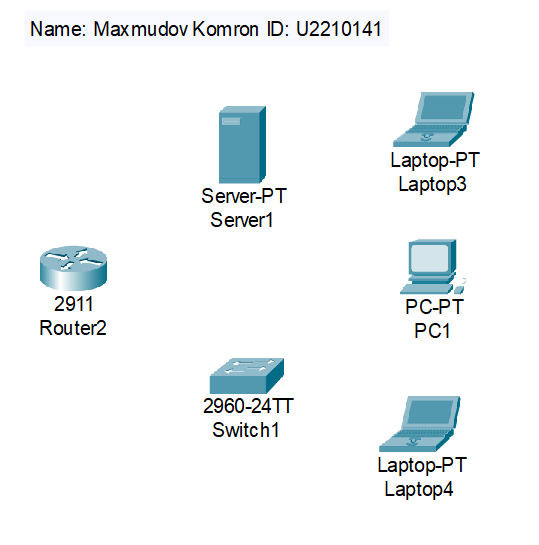
\includegraphics[width=0.8\textwidth]{Images/4.1.png}}

\item \textbf{Configured Router Interface:} I assigned the IP address \texttt{192.168.10.1} with a subnet mask of \texttt{255.255.255.0} to the router’s \texttt{GigabitEthernet 0/0} interface and enabled it to act as the default gateway for the network.

\fbox{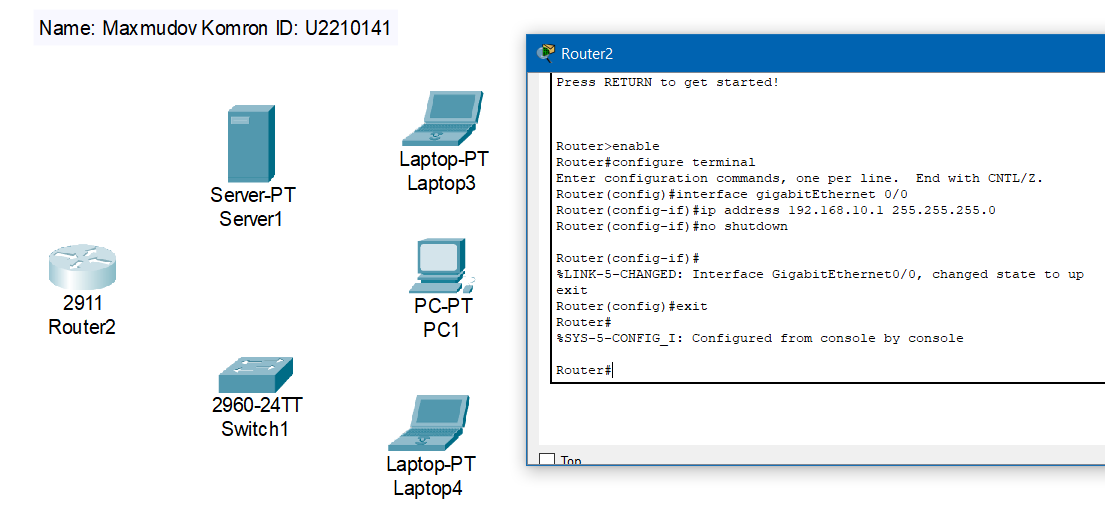
\includegraphics[width=0.8\textwidth]{Images/4.2.png}}

\item \textbf{Configured DHCP Server:} On the DHCP server, I opened the \texttt{Services} tab, selected \texttt{DHCP}, and created a DHCP pool with the following parameters:
\begin{itemize}
  \item Default Gateway: \texttt{192.168.10.1}
  \item Subnet Mask: \texttt{255.255.255.0}
  \item DNS Server: \texttt{8.8.8.8}
  \item Starting IP Address: \texttt{192.168.10.10}
  \item Maximum Number of Users: 50
\end{itemize}

\fbox{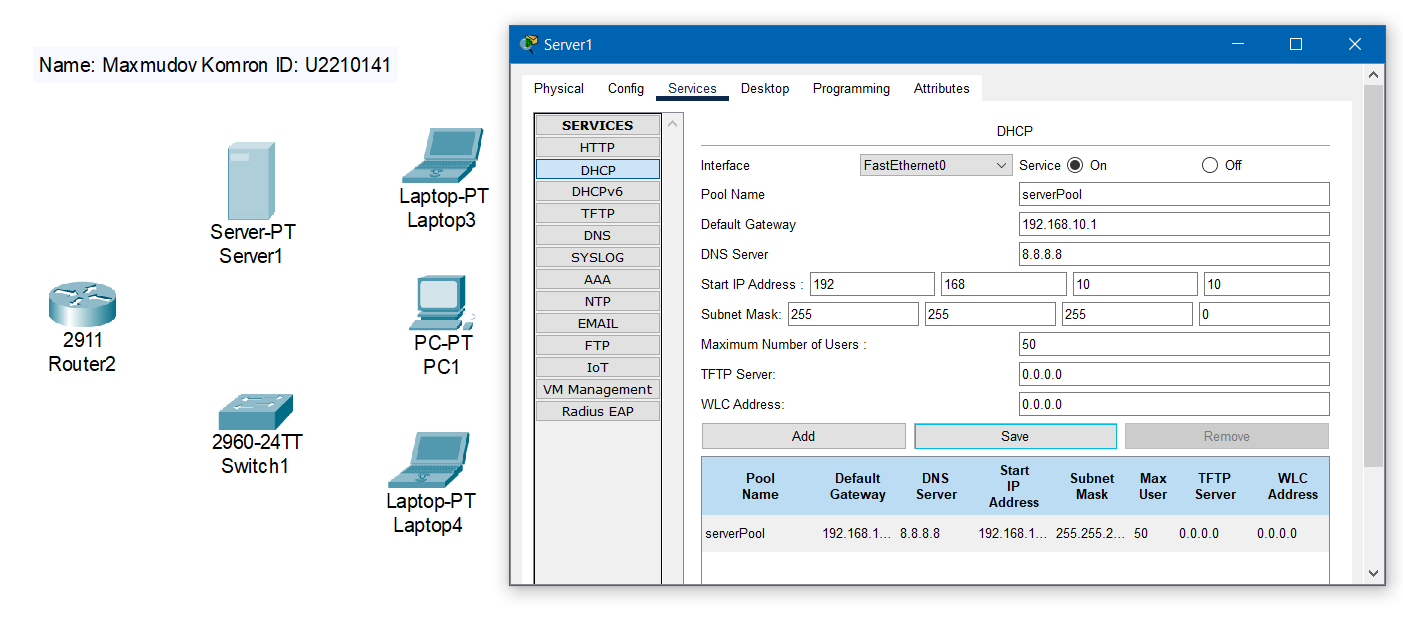
\includegraphics[width=0.8\textwidth]{Images/4.3.png}}

\item \textbf{Connected All Devices:} I connected the router, DHCP server, and end devices to the switch using copper straight-through cables. This ensured all devices, including the DHCP server, were on the same subnet and broadcast domain, allowing DHCP requests to reach the server directly without routing.

\fbox{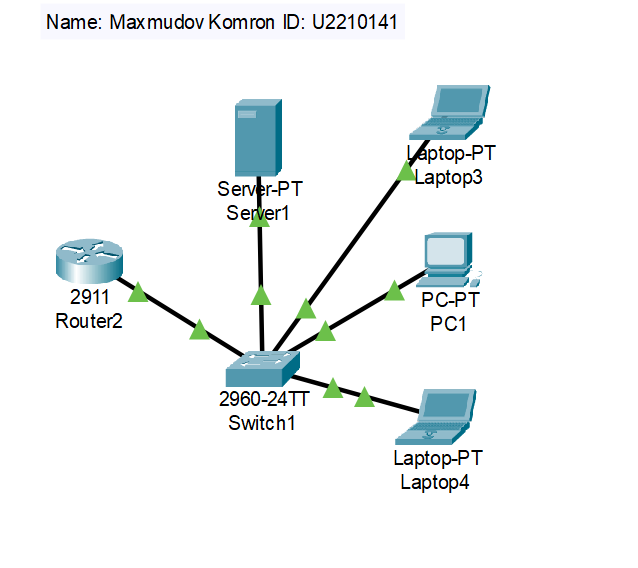
\includegraphics[width=0.8\textwidth]{Images/4.4.png}}

\item \textbf{Enabled DHCP on End Devices:} I opened the IP configuration on each PC and laptop, set them to obtain an IP address automatically, and verified that each device received an IP address from the DHCP server within the specified range.

\fbox{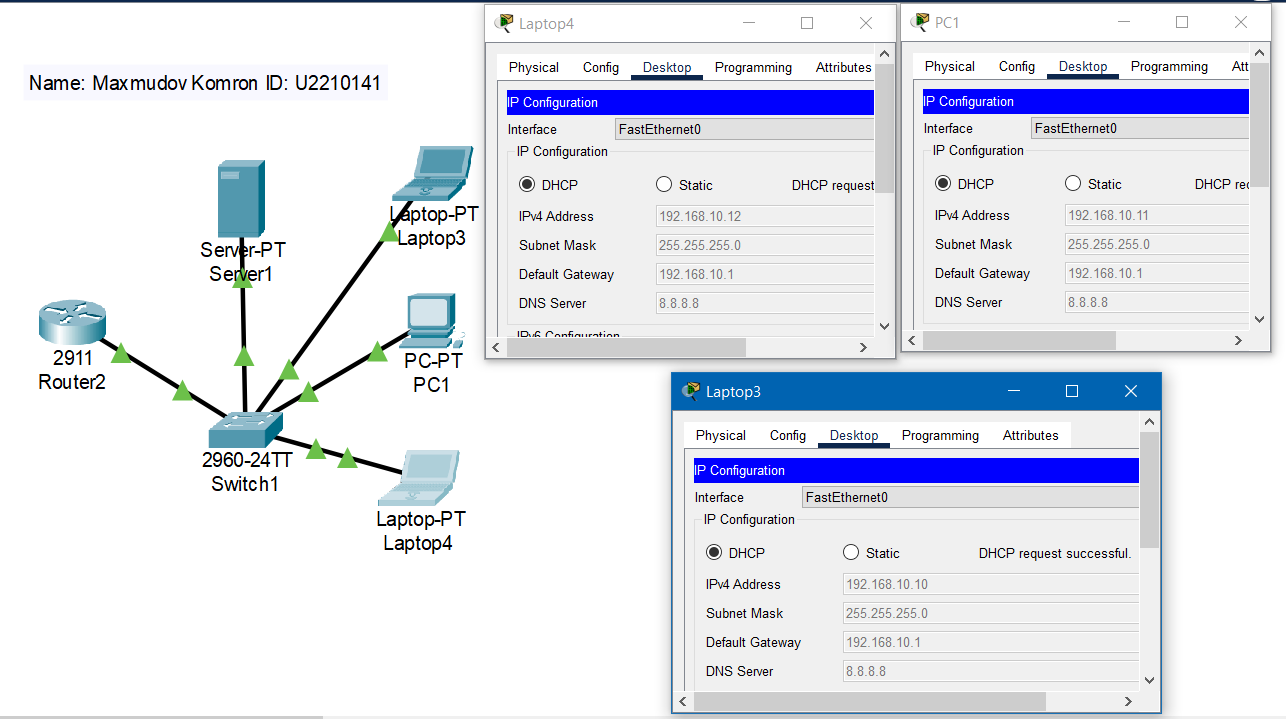
\includegraphics[width=0.8\textwidth]{Images/4.5.png}}

\item \textbf{Tested Network Connectivity:} I used the \texttt{ping} command between end devices and to the default gateway to confirm successful IP assignment and ensure that all devices were able to communicate over the network.

\fbox{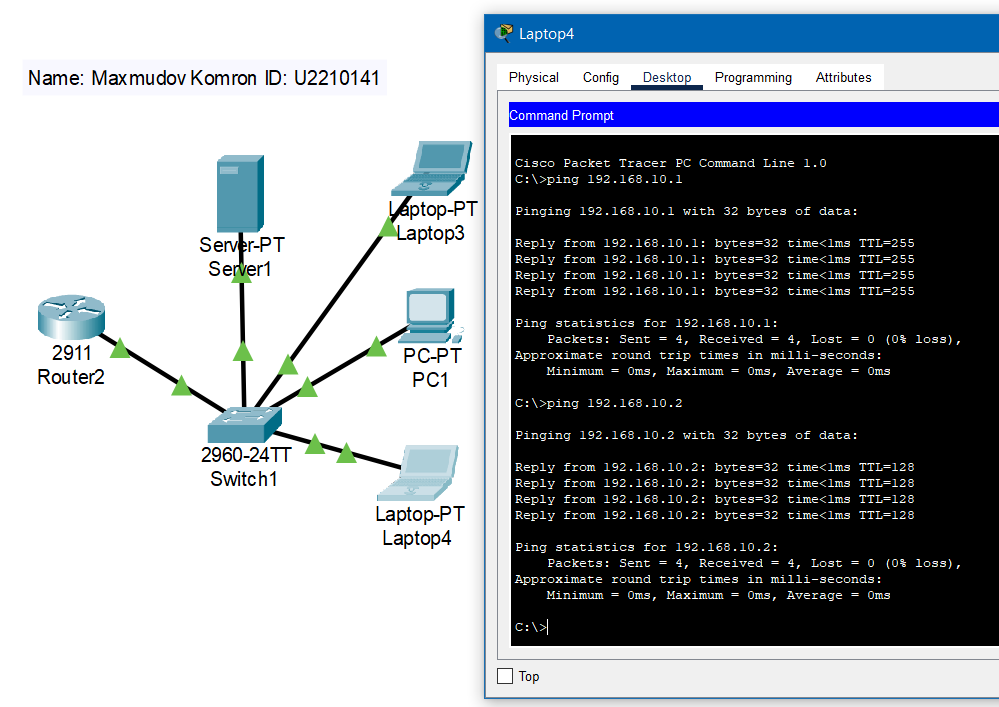
\includegraphics[width=0.8\textwidth]{Images/4.6.png}}
\end{enumerate}

\subsection{Summary}

In this activity, I successfully configured a dedicated DHCP server to automatically assign IP addresses to multiple client devices on a network. The DHCP server was connected to the switch along with all end devices, ensuring they shared the same local network. The router was configured as the default gateway. All devices were able to obtain their addresses dynamically and communicate with each other, confirming correct DHCP setup and full network connectivity.

\section{Activity 5 – Simulate FTP Server using Cisco Packet Tracer}

\subsection{Concept Overview}

A \textbf{File Transfer Protocol (FTP) Server} is used for sharing and transferring files over a network. It allows client devices to connect to a centralized server and perform file operations such as uploading and downloading using FTP commands. In this activity, I simulated an FTP server in Cisco Packet Tracer, where PCs were configured to access and interact with the server.

\subsection{Simulation Steps}

\begin{enumerate}
\item \textbf{Created Network Topology and Connected Devices:} I placed a server, a switch, and two PCs in the Cisco Packet Tracer workspace to simulate a simple LAN-based FTP network. I used copper straight-through cables to connect all devices to the switch as follows:
\begin{itemize}
  \item Server \textrightarrow{} Switch 
  \item PC0 \textrightarrow{} Switch  
  \item PC1 \textrightarrow{} Switch
\end{itemize}

\fbox{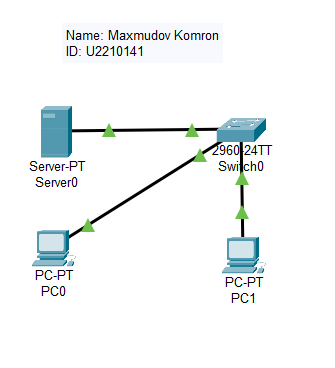
\includegraphics[width=0.8\textwidth]{Images/5.1.png}}

\item \textbf{Assigned IP Addresses:} I manually configured IP addresses for all devices in the same subnet:
\begin{itemize}
  \item Server: \texttt{192.168.10.2}, Subnet Mask: \texttt{255.255.255.0}
  \item PC0: \texttt{192.168.10.10}, Subnet Mask: \texttt{255.255.255.0}
  \item PC1: \texttt{192.168.10.11}, Subnet Mask: \texttt{255.255.255.0}
\end{itemize}

\fbox{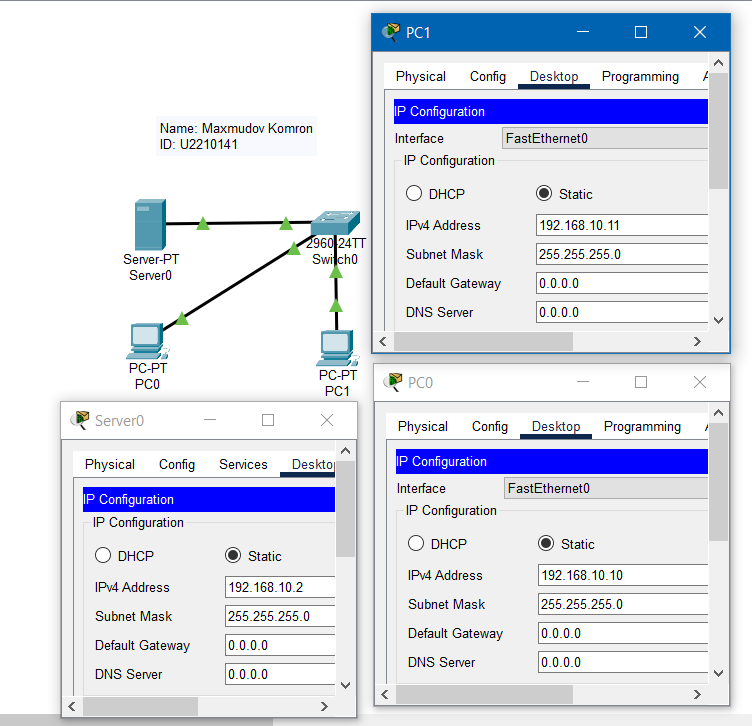
\includegraphics[width=0.8\textwidth]{Images/5.2.png}}

\item \textbf{Configured FTP Service on Server:} I opened the \texttt{Services} tab on the server, selected \texttt{FTP}, turned the service ON, and created a user with login credentials:
\begin{itemize}
  \item Username: \texttt{ftpuser}
  \item Password: \texttt{Kama123}
\end{itemize}

\fbox{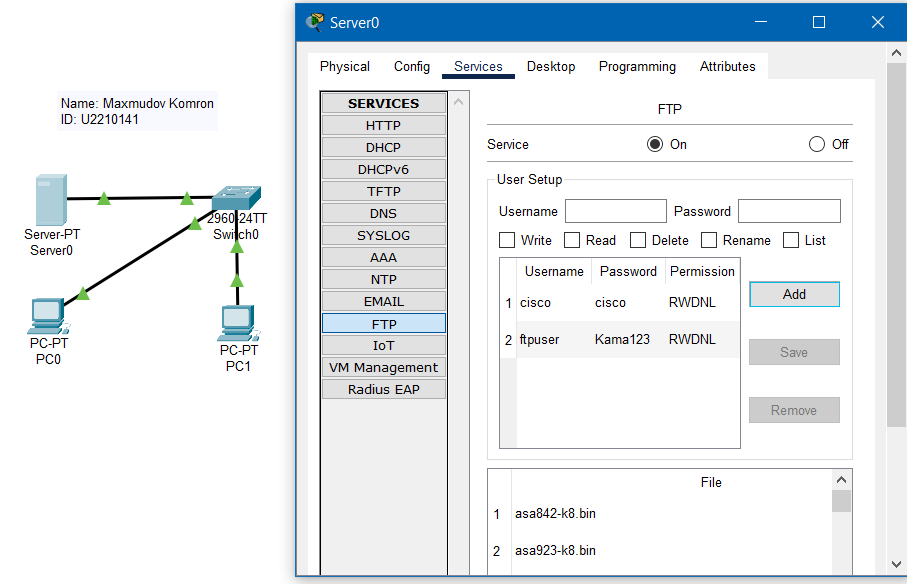
\includegraphics[width=0.8\textwidth]{Images/5.3.png}}

\item \textbf{Tested FTP from PC:} I opened the \texttt{Command Prompt} on PC0 and typed:
\begin{verbatim}
ftp 192.168.10.2
\end{verbatim}
Then I logged in using the created username and password to access the server.

\fbox{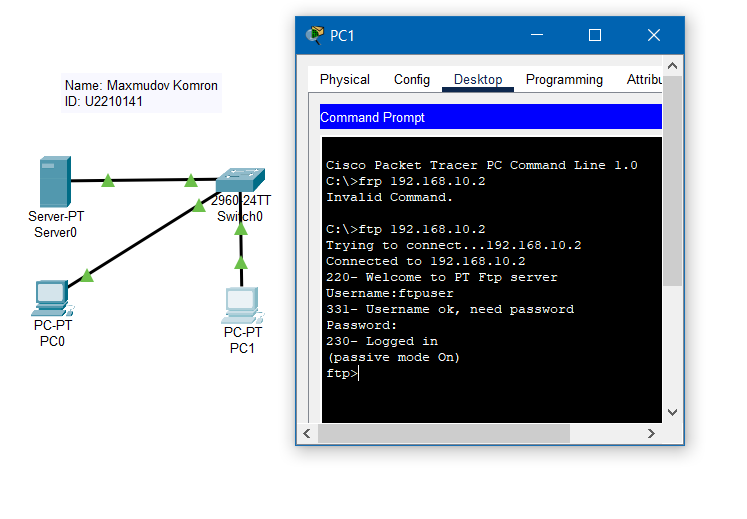
\includegraphics[width=0.8\textwidth]{Images/5.4.png}}

\item \textbf{Transferred Files Using FTP Commands:} After successful login, I used FTP commands such as:
\begin{itemize}
  \item \texttt{dir} – to list server files
  \item \texttt{get filename} – to download files
  \item \texttt{put filename} – to upload files
  \item \texttt{bye} – to close the session
\end{itemize}

\fbox{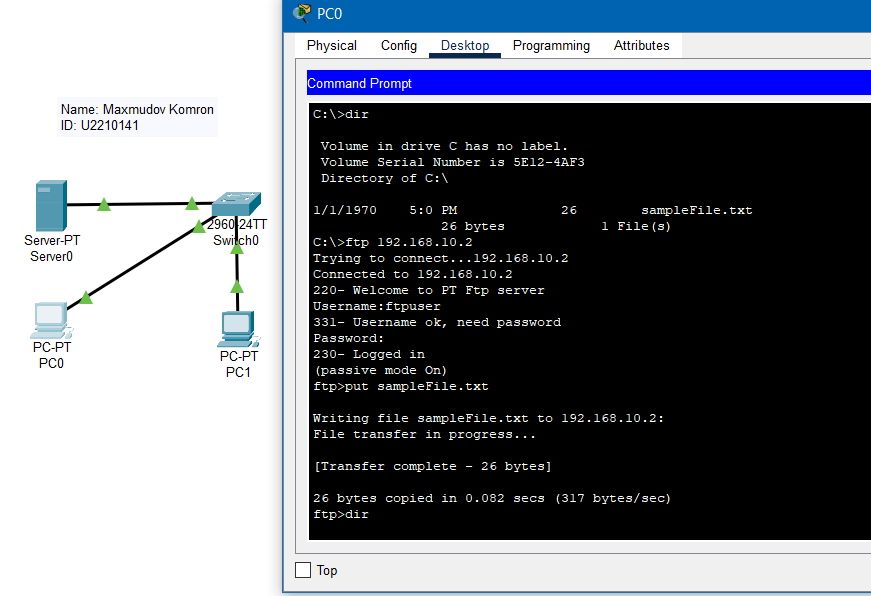
\includegraphics[width=0.8\textwidth]{Images/5.5.1.png}} \\[1em]
\fbox{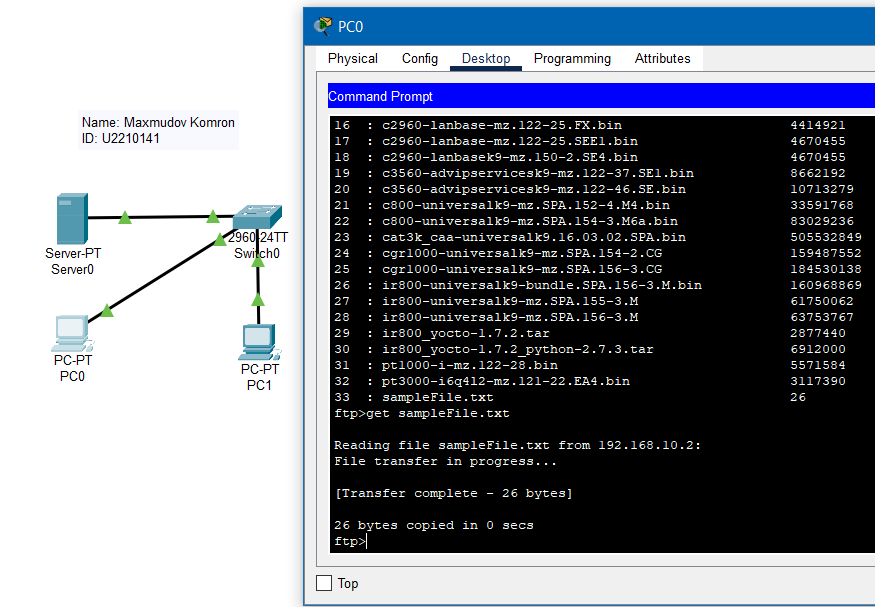
\includegraphics[width=0.8\textwidth]{Images/5.5.2.png}}

\end{enumerate}

\subsection{Summary}

In this activity, I simulated a basic FTP network in Cisco Packet Tracer using a server and two PCs connected through a switch. After enabling the FTP service and creating user credentials, I tested connectivity and successfully uploaded and downloaded files using FTP commands from the PCs. This activity demonstrated how FTP works in a local network environment for file sharing.

\section{Activity 6 – HTTP Web Server Configuration using Cisco Packet Tracer}

\subsection{Concept Overview}
A \textbf{Hypertext Transfer Protocol (HTTP) Web Server} is used to host and serve web pages to clients over a network. Web browsers (clients) request web pages from the server using HTTP, and the server responds by delivering the requested content. In this activity, I configured an HTTP web server in Cisco Packet Tracer and accessed it using a web browser from client PCs.

\subsection{Simulation Steps}
\begin{enumerate}

\item \textbf{Created Network Topology and Connected Devices:}  
I placed a server, a switch, and two PCs in the Cisco Packet Tracer workspace to simulate a simple LAN-based web network. Copper straight-through cables were used to connect all devices to the switch:
\begin{itemize}
  \item Server \textrightarrow{} Switch
  \item PC0 \textrightarrow{} Switch
  \item PC1 \textrightarrow{} Switch
\end{itemize}

\fbox{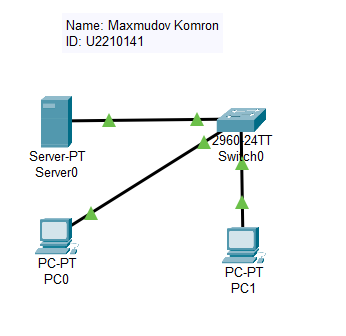
\includegraphics[width=0.8\textwidth]{Images/6.1.png}}

\item \textbf{Assigned IP Addresses:}  
Each device was manually assigned an IP address in the same subnet:
\begin{itemize}
  \item Server: \texttt{192.168.10.2}, Subnet Mask: \texttt{255.255.255.0}
  \item PC0: \texttt{192.168.10.10}, Subnet Mask: \texttt{255.255.255.0}
  \item PC1: \texttt{192.168.10.11}, Subnet Mask: \texttt{255.255.255.0}
\end{itemize}

\fbox{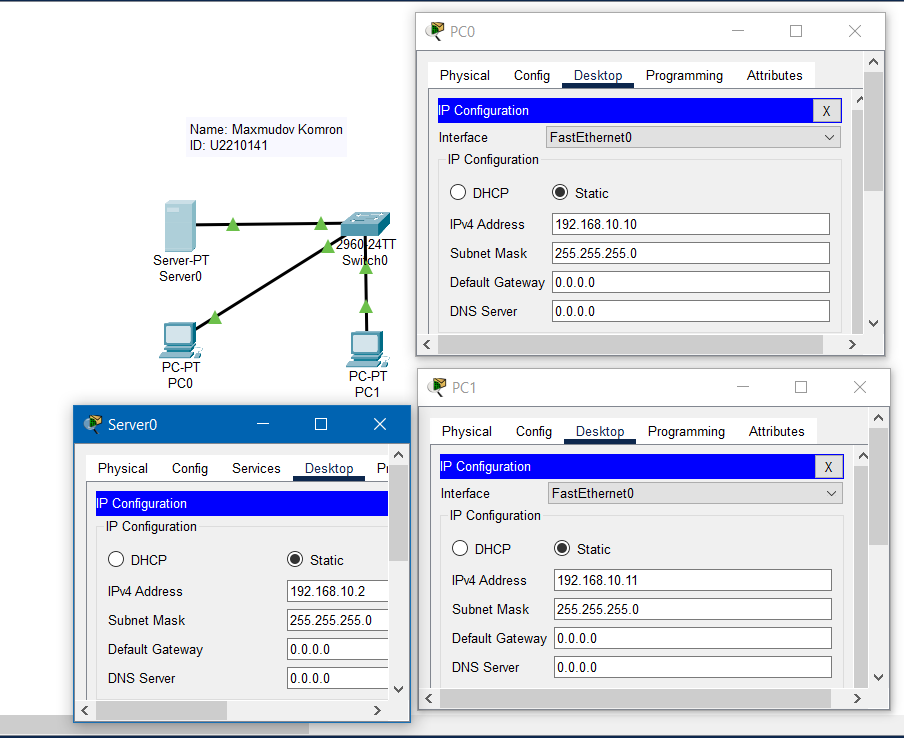
\includegraphics[width=0.8\textwidth]{Images/6.2.png}}

\item \textbf{Configured HTTP Service on the Server:}  
I opened the \textbf{Services} tab on the server, selected \textbf{HTTP}, and turned the service ON.

\fbox{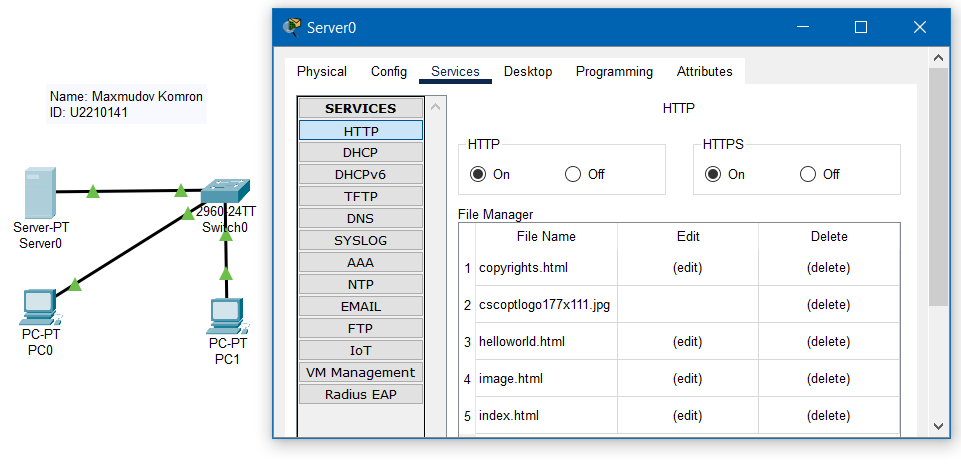
\includegraphics[width=0.8\textwidth]{Images/6.3.png}}

\item \textbf{Accessed the Web Page from PC0:}  
On PC0, I opened the web browser and entered the server’s IP address in the URL bar:
\begin{verbatim}
http://192.168.10.2
\end{verbatim}
The default web page hosted on the server was successfully displayed.

\fbox{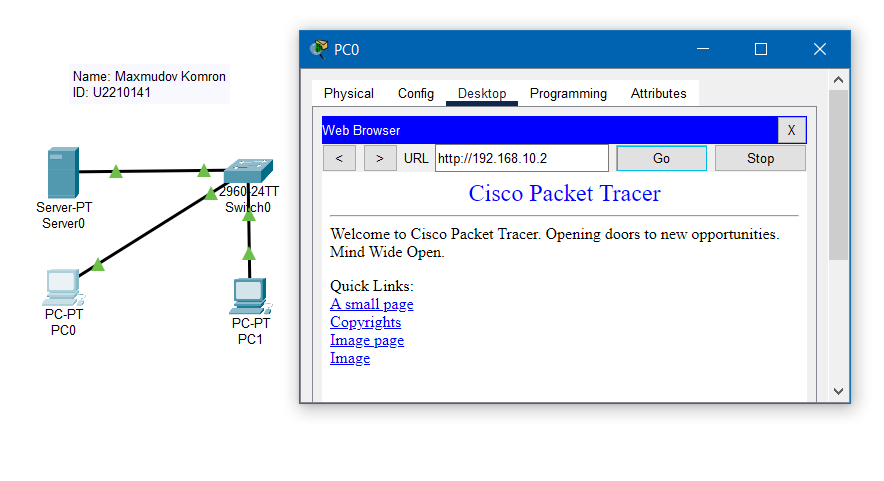
\includegraphics[width=0.8\textwidth, trim=0 50 0 0, clip]{Images/6.4.png}}

\item \textbf{Customized the Web Page:}  
I modified the default web page by navigating to the \textbf{HTTP} service tab on the server and editing the default \texttt{index.html} file. After saving the changes, I refreshed the browser on PC0 to verify the update.

\fbox{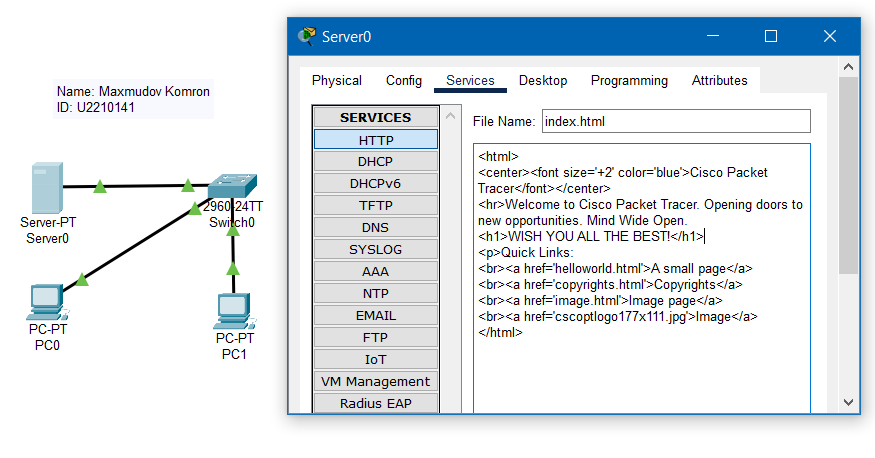
\includegraphics[width=0.8\textwidth]{Images/6.5.1.png}} \\[1em]
\fbox{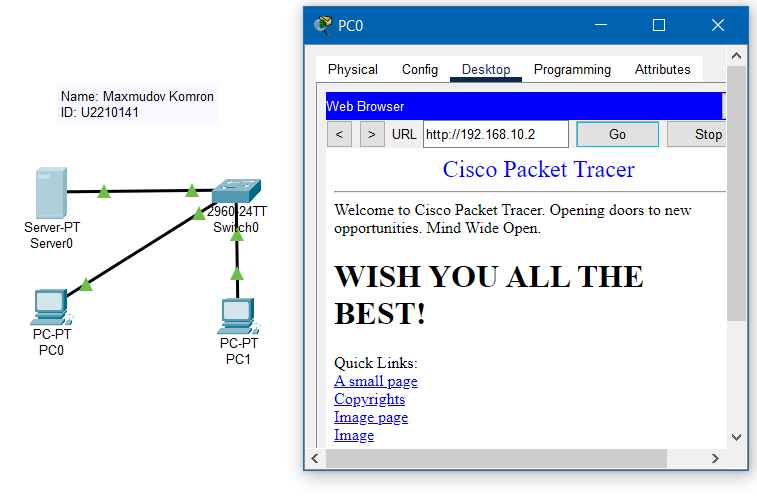
\includegraphics[width=0.8\textwidth]{Images/6.5.2.png}}

\end{enumerate}

\subsection{Summary}
In this activity, I simulated an HTTP web server in Cisco Packet Tracer and connected two PCs through a switch. After enabling the HTTP service on the server, I accessed the hosted web page from a web browser on PC0. Additionally, I modified the web page’s content and verified the changes in real-time. This activity demonstrated how a basic web server operates within a local network.

\section{Activity 7 – Subnetting and Network Design in Cisco Packet Tracer}

\subsection{Concept Overview}
In this activity, I was given the IP block \texttt{130.34.12.64/26} and required to divide it into four equal subnetworks. To efficiently implement this design, I used VLAN segmentation and a single-router interface configured with subinterfaces (Router-on-a-Stick). This approach is both scalable and resource-efficient, offering full inter-subnet communication while minimizing physical complexity.

\begin{table}[h!]
\centering
\begin{tabular}{|c|c|c|c|}
\hline
\textbf{Subnet} & \textbf{Network Address} & \textbf{Range} & \textbf{Broadcast Address} \\
\hline
Subnet 1 & 130.34.12.64/28 & 130.34.12.65 – 130.34.12.78 & 130.34.12.79 \\
Subnet 2 & 130.34.12.80/28 & 130.34.12.81 – 130.34.12.94 & 130.34.12.95 \\
Subnet 3 & 130.34.12.96/28 & 130.34.12.97 – 130.34.12.110 & 130.34.12.111 \\
Subnet 4 & 130.34.12.112/28 & 130.34.12.113 – 130.34.12.126 & 130.34.12.127 \\
\hline
\end{tabular}
\vspace{0.5em}
\captionsetup{justification=centering}
\caption{Subnet Division of \texttt{130.34.12.64/26} into Four \texttt{/28} Networks}
\end{table}

\subsection{Simulation Steps}
\begin{enumerate}

\item \textbf{Built the Network Topology:} I placed one router, one switch, and eight PCs (two per subnet). All PCs were connected to the same switch. The switch was then connected to the router's \texttt{GigabitEthernet0} interface using a trunk link.

\fbox{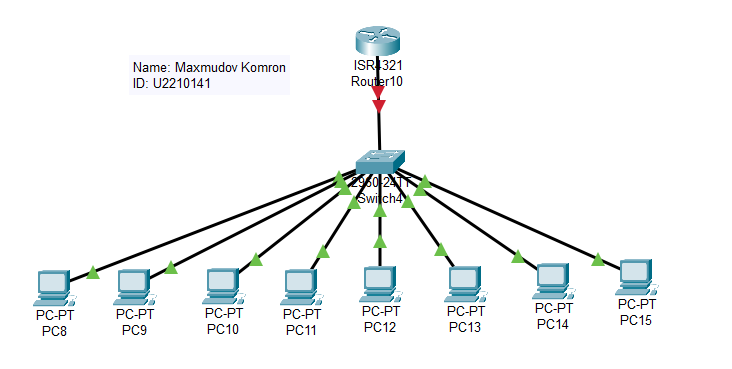
\includegraphics[width=0.8\textwidth]{Images/7.1.png}}

\item \textbf{Configured VLANs on the Switch:} I created four VLANs (10, 20, 30, 40), one for each subnet. Each VLAN contained two PCs. Access ports were assigned based on VLAN membership, and the switch port connected to the router was configured as a trunk port to allow VLAN-tagged traffic.

\fbox{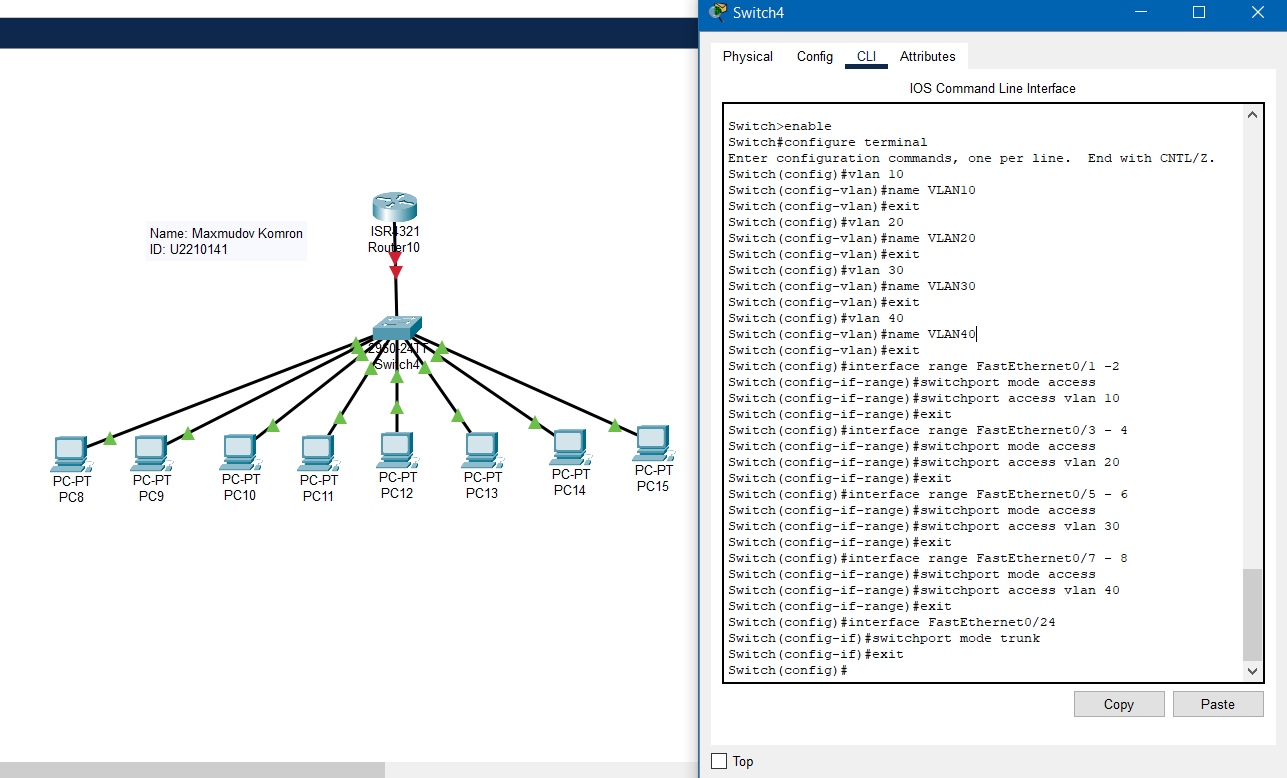
\includegraphics[width=0.8\textwidth]{Images/7.2.png}}

\item \textbf{Configured Router Subinterfaces:} I created four subinterfaces under \texttt{GigabitEthernet0}, each configured with 802.1Q encapsulation for its corresponding VLAN. Each subinterface was assigned an IP address from its respective subnet, serving as the default gateway for that VLAN.

\fbox{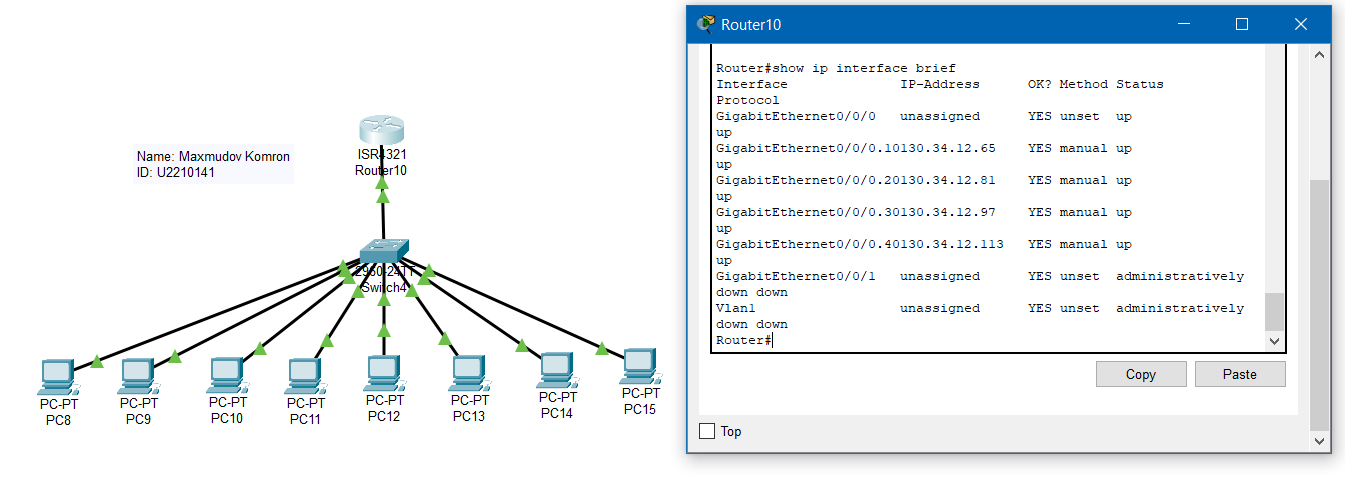
\includegraphics[width=0.8\textwidth]{Images/7.3.png}}

\item \textbf{Assigned IP Addresses to PCs:} Each PC was manually configured with an IP address, subnet mask, and default gateway according to its VLAN’s subnet. This ensured accurate IP addressing and gateway communication.

\fbox{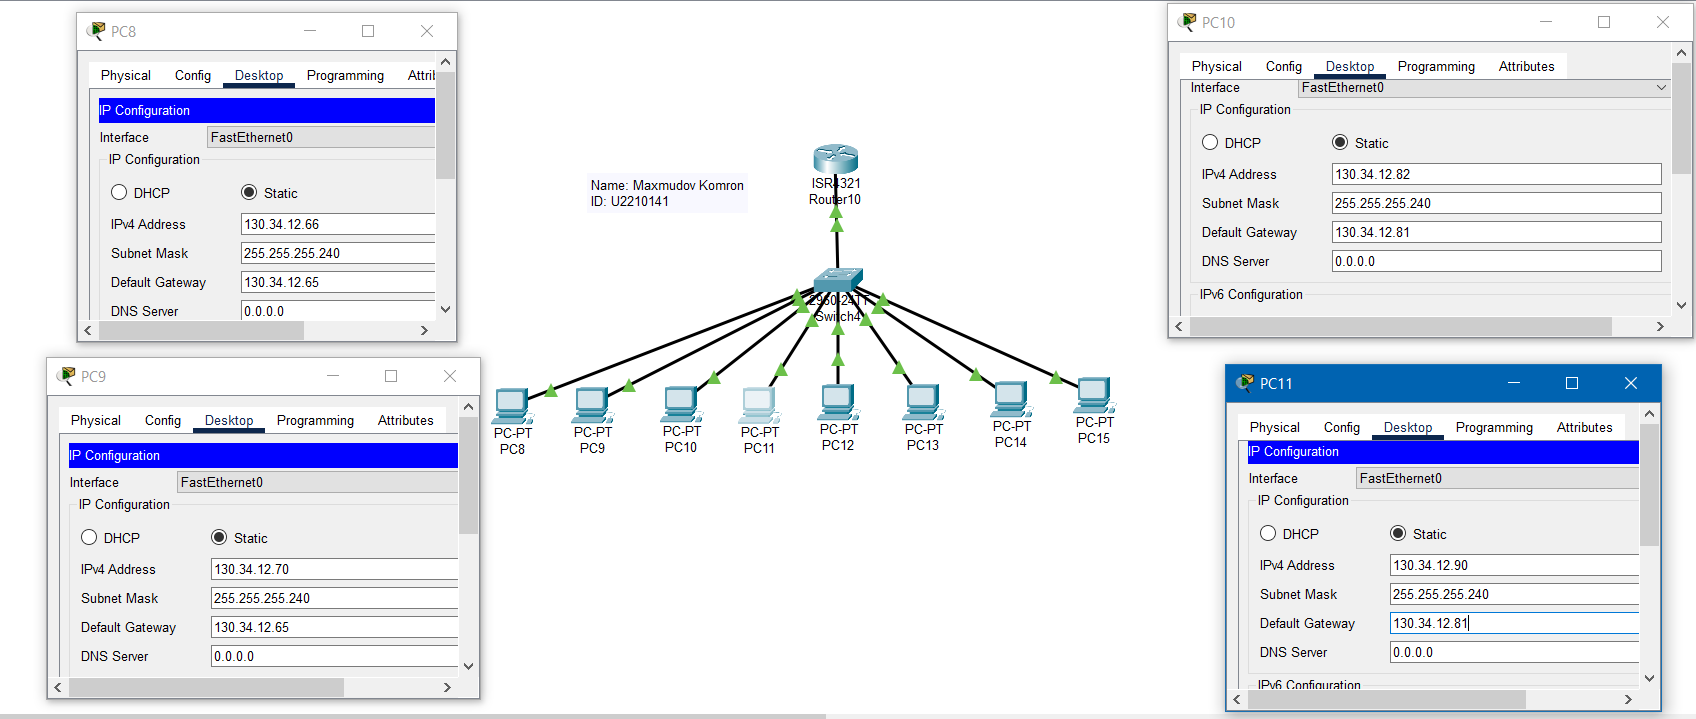
\includegraphics[width=0.8\textwidth]{Images/7.4.png}}

\item \textbf{Tested Connectivity:} I verified communication within VLANs by pinging between PCs in the same subnet. Then, I tested inter-VLAN routing by pinging across different VLANs. All connectivity tests were successful, demonstrating proper routing and subnetting.

\fbox{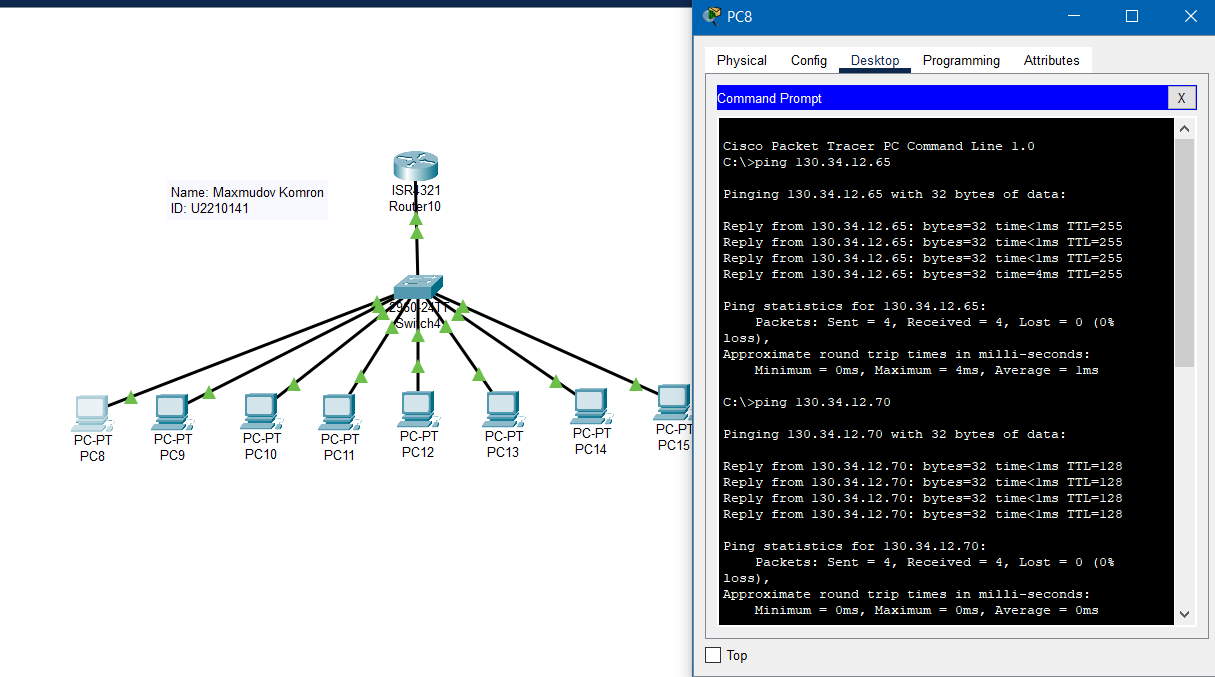
\includegraphics[width=0.8\textwidth]{Images/7.5.1.png}} \\[1em]
\fbox{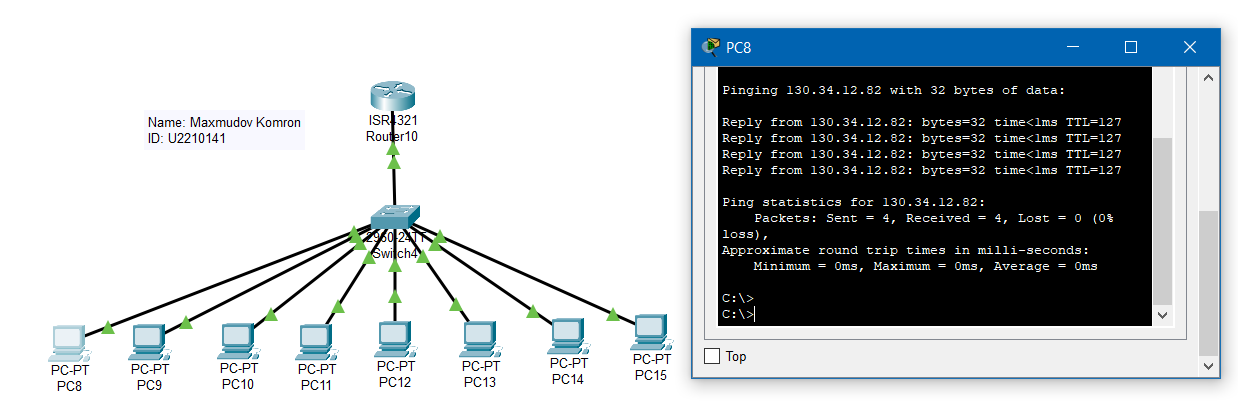
\includegraphics[width=0.8\textwidth]{Images/7.5.2.png}}
\end{enumerate}

\subsection{Summary} 

In this activity, I subnetted the \texttt{/26} network into four equal \texttt{/28} subnetworks and implemented a VLAN-based topology using Router-on-a-Stick. This design reduced hardware requirements, centralized routing, and maintained clear separation between subnetworks. The approach allowed efficient IP address management, reliable routing, and ensured all end devices could communicate across subnet boundaries.

\section{Activity 8 – Distance Vector Routing using RIP Protocol}

\subsection{Concept Overview}
In this activity, I demonstrated the principles of Distance Vector Routing by implementing the Routing Information Protocol (RIP) in a simulated network with two routers. RIP is a dynamic routing protocol that uses hop count as its metric and operates through periodic updates and routing table advertisements. This activity helped reinforce concepts such as dynamic route learning, hop count metrics, and route convergence.

\subsection{Simulation Steps}
\begin{enumerate}

\item \textbf{Built the Network Topology:} I created a network with two routers (Router22 and Router23), each connected to its own local network of end devices via a switch. Router22 is connected to PC10 and PC11; Router23 is connected to Laptop4 and Laptop5. The routers are connected through a serial cable.

\fbox{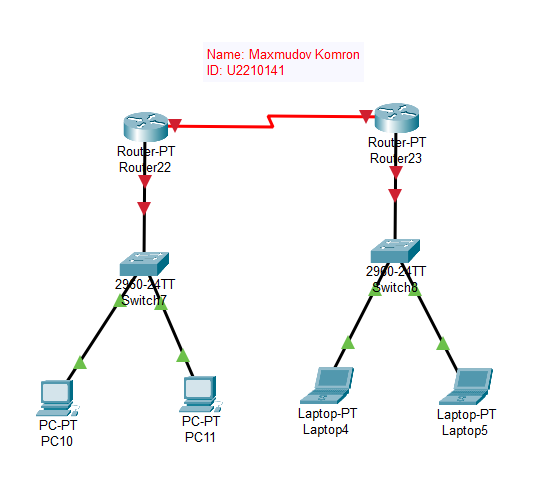
\includegraphics[width=0.8\textwidth]{Images/8.1.png}} 

\item \textbf{Assigned IP Addresses:} I manually assigned IP addresses to each PC, laptop, and router interface. Each subnet was given a unique IP block. For example, Router22's LAN used 192.168.10.0/24, Router23's LAN used 192.168.20.0/24, and the serial link used 10.0.0.0/30.

\fbox{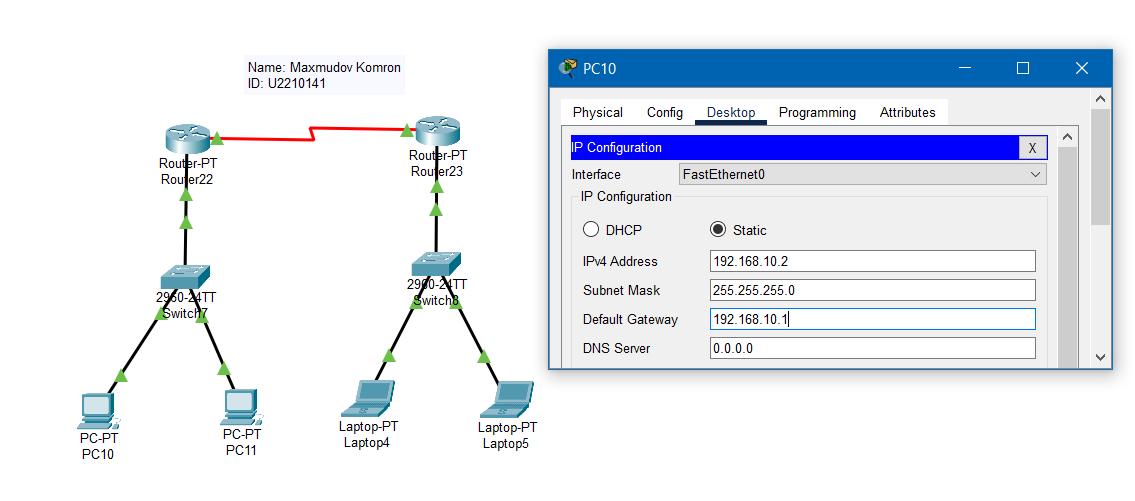
\includegraphics[width=0.8\textwidth]{Images/8.2.png}}

\item \textbf{Enabled RIP on Routers:} On both routers, I enabled RIP version 2 and advertised all directly connected networks. This allowed the routers to dynamically learn about remote subnets through periodic updates.

\fbox{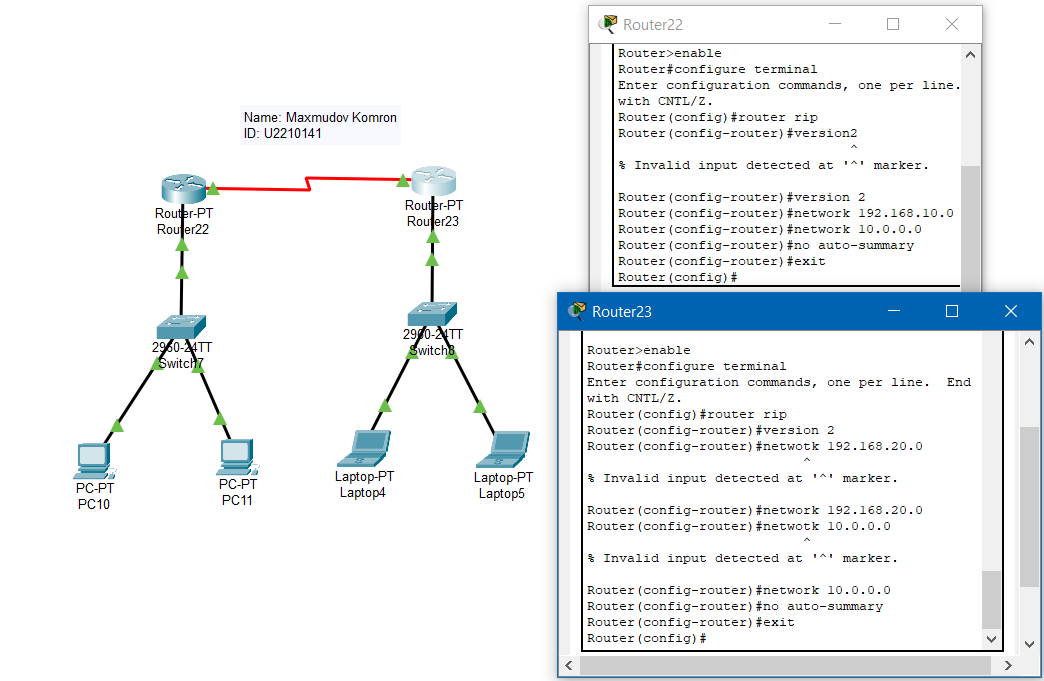
\includegraphics[width=0.8\textwidth]{Images/8.3.png}}

\item \textbf{Verified Routing Tables:} I used the \texttt{show ip route} command on each router to check if routes to remote networks had been learned via RIP. The presence of RIP-learned routes confirmed correct configuration.

\fbox{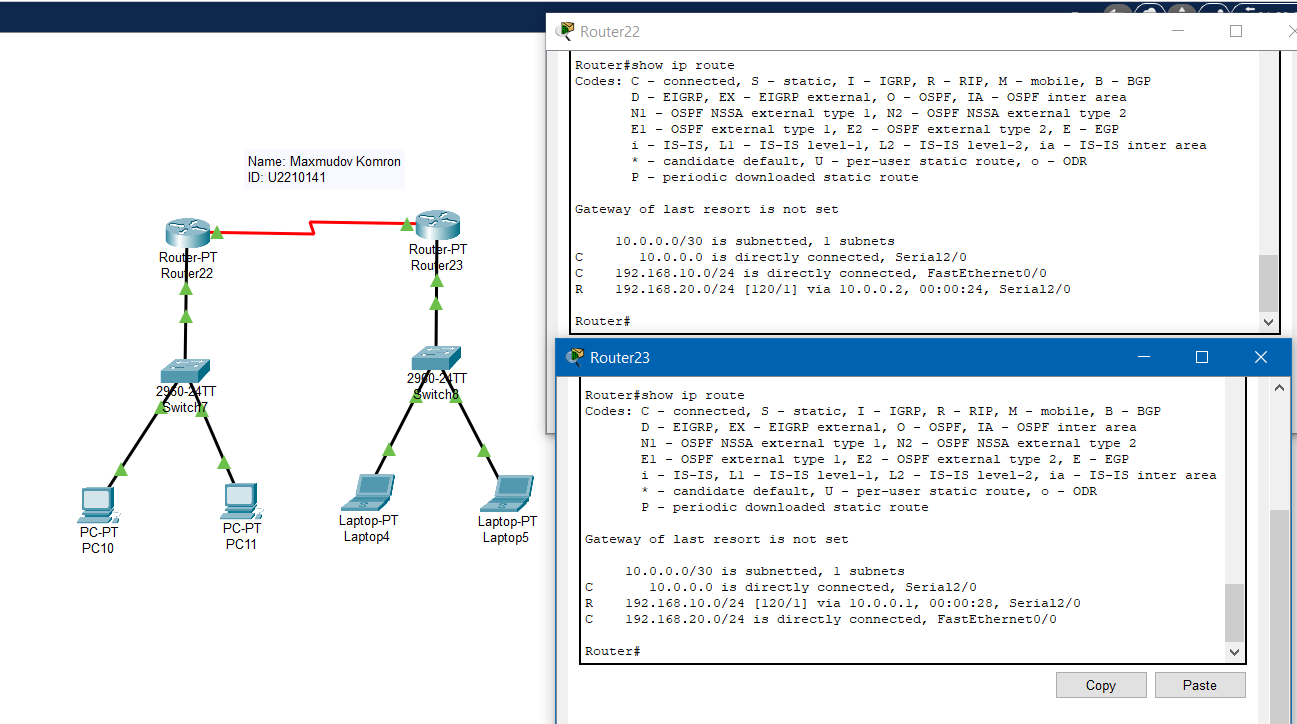
\includegraphics[width=0.8\textwidth]{Images/8.4.png}}

\item \textbf{Tested Connectivity:} I tested connectivity by pinging from PC10 (in Router22’s network) to Laptop4 (in Router23’s network). Successful pings confirmed that the RIP protocol propagated the necessary routes.

\fbox{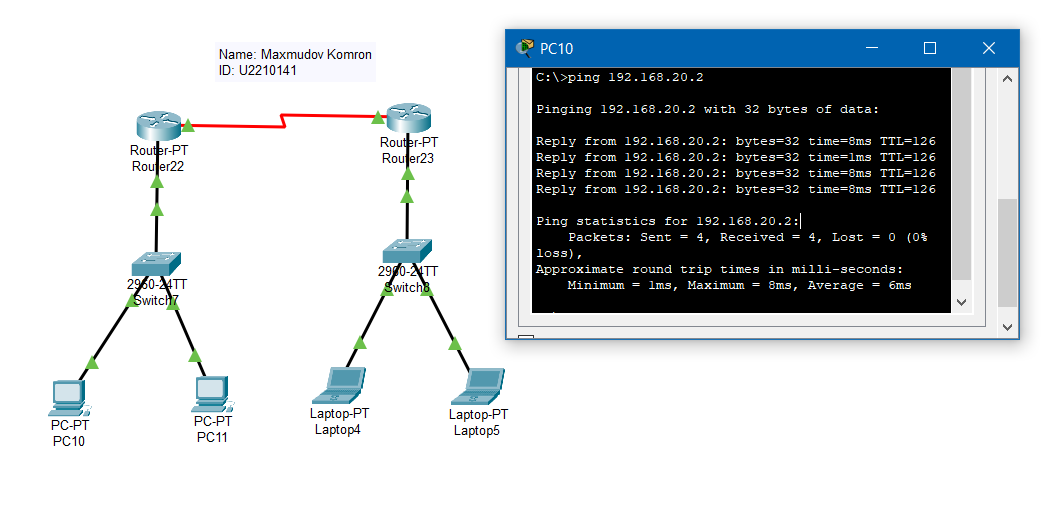
\includegraphics[width=0.8\textwidth]{Images/8.5.png}}

\end{enumerate}

\subsection{Summary}

In this activity, I implemented RIP routing between two routers to allow communication between two LANs. RIP enabled dynamic route exchange, removing the need for manual static routes. I verified the successful configuration by checking routing tables and testing end-to-end connectivity. This hands-on task demonstrated the functionality of RIP’s distance vector mechanism, hop count limitation, and automatic route updates across routers.

\section{Activity 9 – Configuring VLAN and Inter Routing VLAN setup }

\subsection{Concept Overview}
In this activity, I implemented VLAN segmentation and Inter-VLAN routing in Cisco Packet Tracer. VLANs provide logical separation of devices within a switch, improving security and traffic control. Since devices in different VLANs cannot communicate by default, I used a Router-on-a-Stick configuration to enable inter-VLAN communication through router subinterfaces. This design supports centralized routing while maintaining VLAN boundaries.

\subsection{Simulation Steps}
\begin{enumerate}

\item \textbf{Built the Network Topology:} I used one router, one switch, and eight PCs (two per VLAN). All PCs were connected to the same switch, which was linked to the router’s \texttt{GigabitEthernet0} interface via a trunk connection.

\fbox{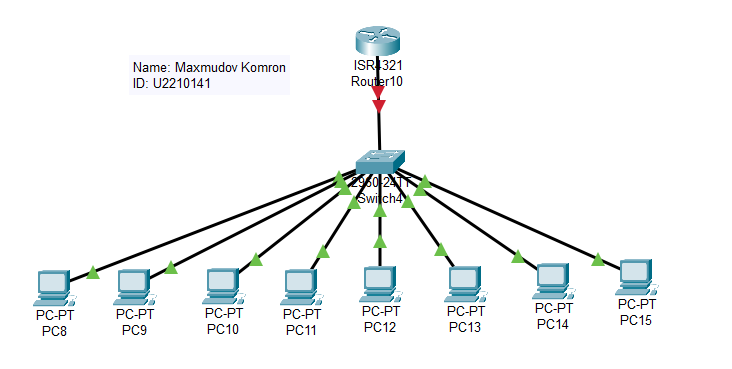
\includegraphics[width=0.8\textwidth]{Images/7.1.png}}

\item \textbf{Configured VLANs on the Switch:} I created four VLANs (10, 20, 30, 40) and assigned each pair of PCs to a separate VLAN. I also configured access ports for end devices and set the router-facing port as a trunk to carry VLAN-tagged traffic.

\fbox{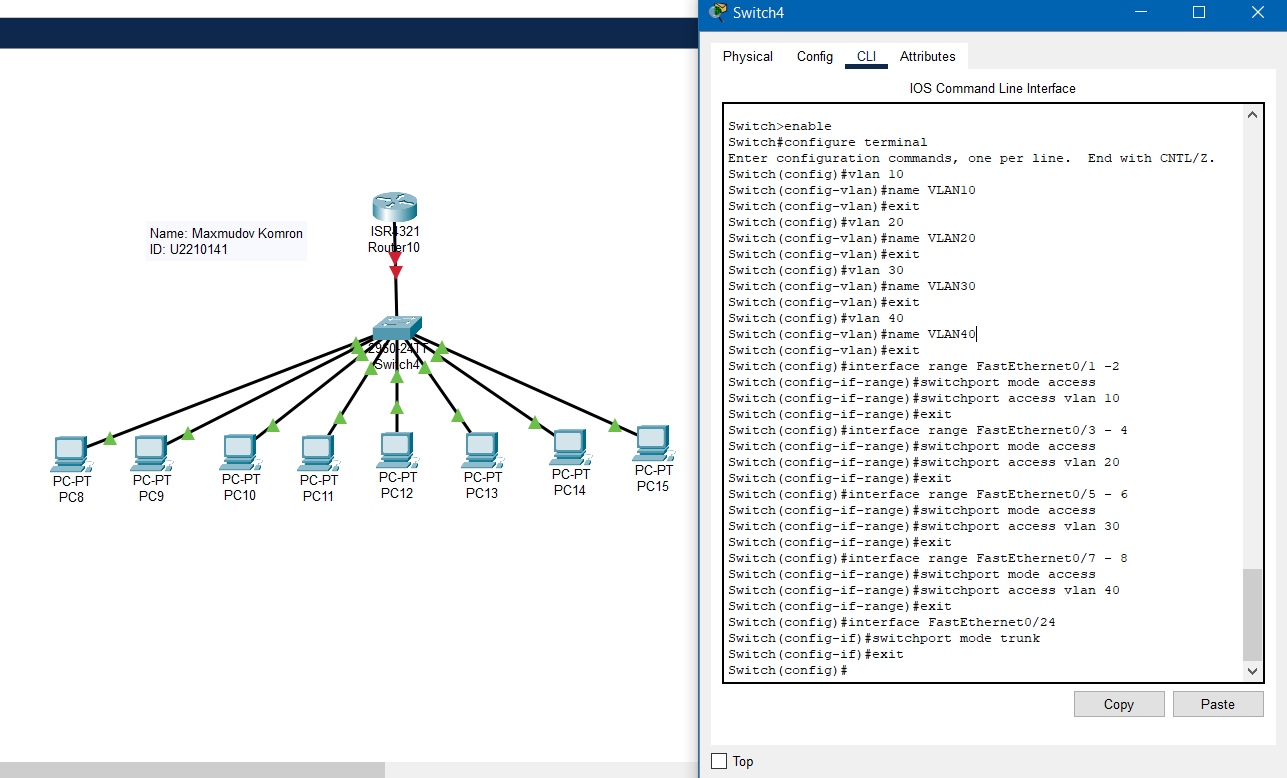
\includegraphics[width=0.8\textwidth]{Images/7.2.png}}

\item \textbf{Configured Router Subinterfaces:} I created four subinterfaces under \texttt{GigabitEthernet0}, each mapped to a VLAN using 802.1Q encapsulation. Each subinterface was assigned a gateway IP address for its VLAN.

\fbox{\includegraphics[width=0.8\textwidth]{Images/7.3.png}}

\item \textbf{Assigned IP Addresses to PCs:} Each PC was configured with a static IP address, subnet mask, and default gateway that matched its VLAN. This ensured proper addressing and gateway communication.

\fbox{\includegraphics[width=0.8\textwidth]{Images/7.4.png}}

\item \textbf{Tested Inter-VLAN Connectivity:} I verified communication within each VLAN by pinging between same-VLAN PCs. Then, I tested inter-VLAN routing by pinging across different VLANs. All tests were successful.

\fbox{\includegraphics[width=0.8\textwidth]{Images/7.5.1.png}} \\[1em]
\fbox{\includegraphics[width=0.8\textwidth]{Images/7.5.2.png}}

\end{enumerate}

\subsection{Summary} 
In this activity, I used VLANs to segment the network and configured a Router-on-a-Stick setup to allow inter-VLAN communication. This approach centralized routing while maintaining logical separation between devices. The final setup demonstrated successful VLAN isolation and routing, suitable for scalable network designs.

\section{Activity 10 – Comprehensive Network Design for a Two-Floor Office Building}

\subsection{Project Overview}
This activity involved the design, simulation, and documentation of a network for a two-story office building. The objective was to ensure secure, segmented, and efficient connectivity across various functional areas, considering both wired and wireless access. I approached this task by analyzing floor-wise needs, determining access policies, and selecting suitable network devices and topology. The final design emphasizes practical implementation, security, scalability, and cost-efficiency.

\subsection{Site Layout and Requirements}

\textbf{First Floor}
\begin{itemize}
    \item \textbf{Reception Area:} Requires wired internet access for handling queries and general business operations.
    \item \textbf{Coffee Shop:} Contains two isolated computers with no internet access. Intended for offline note preparation or internal reference.
    \item \textbf{Waiting Room:} Offers wireless internet access to guests and visitors via a dedicated access point.
\end{itemize}

\textbf{Second Floor}
\begin{itemize}
    \item \textbf{Library:} Includes three desktop computers and a network printer. This zone is restricted from internet access and intended for internal resource sharing.
    \item \textbf{Office Rooms:} Equipped with desktops for employees. Devices are allowed internet access and inter-office communication. Wi-Fi is also provided for personal or mobile use.
\end{itemize}

\subsection{Design Strategy and Decisions}

I adopted a \textbf{hybrid hierarchical design} with both wired and wireless segments. VLANs were implemented for logical separation of departments and access policies. A single router serves as the central gateway and applies ACLs to enforce internet restrictions. The design ensures that:

\begin{itemize}
    \item Internal zones (e.g., Library, Coffee Shop) are fully isolated.
    \item Office zones have internet and internal access.
    \item Visitor access is separated via a guest VLAN with Wi-Fi.
    \item Devices are grouped by function and location for management ease.
\end{itemize}

\subsection{VLAN Plan and IP Addressing}

\begin{table}[h!]
\centering
\begin{tabular}{|c|l|c|l|}
\hline
\textbf{VLAN ID} & \textbf{Zone} & \textbf{Subnet} & \textbf{Purpose} \\
\hline
10 & Office Network & 192.168.10.0/24 & Internet + Intranet access \\
20 & Library & 192.168.20.0/24 & Intranet only, printer sharing \\
30 & Reception & 192.168.30.0/24 & Business internet access \\
40 & Coffee Shop & 192.168.40.0/24 & Isolated, offline access only \\
50 & Guest Wi-Fi & 192.168.50.0/24 & Internet access only, no LAN reach \\
\hline
\end{tabular}
\caption{VLAN and Subnet Design}
\end{table}

\subsection{Access Control and Security Rules}

\textbf{Access Control Lists (ACLs)} were configured on the router to restrict or permit traffic based on zone policies:
\begin{itemize}
    \item VLAN 10 (Office) – Full internet and internal access
    \item VLAN 20 (Library) – No internet; access to printer only
    \item VLAN 30 (Reception) – Internet only; no internal access
    \item VLAN 40 (Coffee Shop) – No external or internal access
    \item VLAN 50 (Guest Wi-Fi) – Internet only; isolated from internal VLANs
\end{itemize}

\subsection{Physical and Logical Design Summary}

\begin{itemize}
    \item \textbf{Router:} Acts as the default gateway for all VLANs and manages ACL enforcement.
    \item \textbf{Switches:} Two 24-port managed switches provide connectivity across floors.
    \item \textbf{Access Points:} One per floor, connected via trunk port for VLAN tagging.
    \item \textbf{Printer:} Connected to library VLAN and shared with library PCs.
\end{itemize}

\subsection{Cost Estimation and Device Breakdown}

\begin{table}[!htbp]
\centering
\begin{tabular}{|l|c|r|}
\hline
\textbf{Item} & \textbf{Quantity} & \textbf{Cost (USD)} \\
\hline
Cisco Router (ISR Series) & 1 & 350 \\
24-port Managed Switch & 2 & 400 \\
Access Points (Dual-Band) & 2 & 200 \\
Desktop Computers & 10 & 6000 \\
Network Printer & 1 & 150 \\
Ethernet Cables and Patch Panels & 1 set & 100 \\
UPS Units & 2 & 300 \\
Rack Mount & 1 & 120 \\
\hline
\textbf{Total Estimated Cost} & & \textbf{6,620 USD} \\
\hline
\end{tabular}
\caption{Table 3: Tentative Cost Estimation}
\end{table}

\subsection{Simulation}

\begin{center}
\fbox{\includegraphics[width=0.8\textwidth]{Images/10.1.png}}\\[1em]
\fbox{\includegraphics[width=0.8\textwidth]{Images/10.2.png}}\\[1em]
\fbox{\includegraphics[width=0.8\textwidth]{Images/10.3.png}}\\[1em]
\fbox{\includegraphics[width=0.8\textwidth]{Images/10.4.png}}\\[1em]
\fbox{\includegraphics[width=0.8\textwidth]{Images/10.5.png}}\\[1em]
\fbox{\includegraphics[width=0.8\textwidth]{Images/10.6.png}}\\[1em]
\fbox{\includegraphics[width=0.8\textwidth]{Images/10.7.png}}
\end{center}


\subsection{Summary and Reflections}

\begin{table}[h!]
\centering
\begin{tabular}{|p{6cm}|p{6cm}|c|}
\hline
\textbf{Requirement} & \textbf{Implementation} & \textbf{Fulfilled} \\
\hline
Employees on second floor can access internet via Wi-Fi and communicate internally & Office VLAN (10) allows both internet and intra-office communication; dedicated AP provided for employees & Yes \\
\hline
Reception desk has internet access for managing business queries & Reception PC connected to VLAN 30 with internet access permitted via ACL & Yes \\
\hline
Library computers can share files and access a printer; no internet access & VLAN 20 configured for Library, ACL blocks internet access, allows internal communication and printer use & Yes \\
\hline
Waiting room has wireless internet for visitors & Guest AP configured on VLAN 50; isolated from internal network using ACLs & Yes \\
\hline
Coffee shop has two isolated computers with no internet or internal access & VLAN 40 applied; ACL denies all traffic outside VLAN 40, isolating the devices completely & Yes \\
\hline
\end{tabular}
\caption{Requirement Fulfillment Matrix}
\end{table}

This project provided a real-world simulation of designing a structured, secure, and functional office network across multiple zones. By applying VLAN segmentation, ACLs, and a layered design, I was able to meet all requirements efficiently. The use of a hybrid model (wired + wireless) ensured flexibility, and the simulation verified full connectivity, isolation, and access control. This activity helped solidify concepts in network planning, implementation, and policy-based security.


\end{document}
